\newcommand{\wts}{\mathbf{w}}

\chapter{Maximum Matching}
In this chapter, we will learn about classical algorithms for computing maximum matching in graphs. In this problem, the input is an undirected graph $G = (V, E, \wts)$ on $n$ vertices and $m$ edges with integer edge weights $\wts: E\rightarrow \{1, \ldots, W\}$. A matching is a set of vertex-disjoint edges, and our goal is to find a matching $M$ in $G$ whose total weight $\wts(M) = \sum_{e\in M}\wts(e)$ is maximized.

%  \mprobst{$= \vecone$? The equiv sign is not defined so far... would be fine but maybe confusing?}

\section{Bipartite Matching}
Let us first study maximum weight matching in bipartite graphs. Assume $G = (V = L\cup R, E, \wts)$ is bipartite with vertices in $L$ and $R$ having no edges in between them, respectively. The basic strategy is augmenting paths. 

\subsection{Unit Edge Weights}

To begin with, let us first consider unit edge weights (that is, $\wts= 1$), we could maintain a matching $M$ and repeatedly finding augmenting paths to increase its size until we reach optimum. More specifically, given any matching $M$, we can apply breath-first search from free vertices and maintain a tree of vertices reachable from free vertices in $L$ via simple alternating paths. In the end, if some free vertices in $R$ are reachable via simple alternating paths, then we can recover an augmenting path. Let us formalize this scheme with more details.

\begin{definition}[augmenting path]
	Given a matching $M$ of $G$, a vertex $v$ is called \emph{free} (with respect to $M$) if $v\notin V(M)$, and \emph{matched} if $v\in V(M)$.
	
	Any simple path $\langle u_1, u_2, \ldots, u_l\rangle$ is called an \emph{alternating path} if it begins with an unmatched vertex and whose edges belong alternately to the $M$ and not to $M$, or more formally:
	\begin{enumerate}
	\item $u_1$ is free.
	\item All edges $(u_{2i-1}, u_{2i})$ are unmatched ($(u_{2i-1}, u_{2i})\notin M$), $\forall 1\leq i\leq l/2$.
	\item All edges $(u_{2i}, u_{2i+1})$ are matched ($(u_{2i}, u_{2i+1})\in M$), $\forall 1\leq i\leq (l-1)/2$.
	\end{enumerate}
	An alternating path $\langle u_1, u_2, \ldots, u_l\rangle$ is an \emph{augmenting path} if $u_l$ is free.
\end{definition}

If we could find an augmenting path $\langle u_1, u_2, \ldots, u_l\rangle$ of $M$, then the edge set $$M' = M\cup \{(u_1, u_2), (u_3, u_4), \ldots, (u_{l-1}, u_l)\}\setminus \{(u_2, u_3), (u_4, u_5), \ldots, (u_{l-2}, u_{l-1})\}$$ would be a matching of size $|M|+1$. We argue that augmenting paths always exist whenever $M$ is not maximum.
\begin{lemma}
	If $M$ is not a maximum matching, then there exists an augmenting path with respect to $M$.
\end{lemma}
\begin{proof}
	Let $M^\star$ be the maximum matching of $G$. Then, in the graph $(V, M\cup M^\star)$, all vertices have degree at most $2$, and hence this graph is a union of simple cycles and paths. In each cycle $C$, $M\cap C$ and $M^\star\cap C$ have equal size, and in each path $P$, the sizes of $M\cap P$ and $M^\star\cap P$ differ by at most $1$. Since $|M^\star| > |M|$, there must exist a path $P$ in $(V, M\cup M^\star)$ where $|M^\star\cap P| = |M\cap P|+1$ which would be an augmenting path.
\end{proof}

In bipartite graphs, any augmenting path starting at a free vertex in $L$ should terminate at a free vertex in $R$. To efficiently find an augmenting path, we reduce this task to a reachability problem on a directed graph. More specifically, build a directed graph $\overrightarrow{G}$ as following.
\begin{enumerate}
	\item Start with $G$, and for edges $(u, v)\notin M$, assign a direction from $L$ to $R$, and for edges $(u, v)\in M$, assign a direction from $R$ to $L$.
	
	\item Add an auxiliary source and terminal $s, t$ to $\overrightarrow{G}$. For each free vertex $u\in L$, add a directed edge $(s, u)$ to $\overrightarrow{G}$; symmetrically, for each free vertex $v\in R$, add a directed edge $(v, t)$ to $\overrightarrow{G}$.
\end{enumerate}

\begin{lemma}
	Augmenting paths exist if $s$ can reach $t$ in $\overrightarrow{G}$.
\end{lemma}
\begin{proof}
	Let $\langle s, u_1, u_2, \ldots, u_l, t\rangle$ be a simple directed path from $s$ to $t$ in $\overrightarrow{G}$, then by definition $\langle u_1, u_2, \ldots, u_l\rangle$ is an augmenting path.
\end{proof}

The whole algorithm for unweighted bipartite matching can be summarized as the following pseudo-code \Cref{bipartite-mcm}.

\begin{algorithm}
	\caption{maximum matching in bipartite graph $G = (L\cup R, E)$}\label{bipartite-mcm}
	initialize $M\leftarrow \emptyset$\;
	\Repeat{
		build directed graph $\overrightarrow{G}$\;
		\If{$s$ can reach $t$ in $\overrightarrow{G}$}{
			let $\langle s, u_1, u_2, \ldots, u_l, t\rangle$ be a simple directed path from $s$ to $t$ in $\overrightarrow{G}$\;
			update $M\leftarrow M\cup \{(u_1, u_2), (u_3, u_4), \ldots, (u_{l-1}, u_l)\}\setminus \{(u_2, u_3), (u_4, u_5), \ldots, (u_{l-2}, u_{l-1})\}$\;
		}\Else{
			\textbf{break}\;
		}
	}
	\Return $M$\;
\end{algorithm}

\paragraph{Alternate description of augmenting path searching.} As will be useful for future extensions to non-bipartite graphs, we present here an alternate explanation of how augmenting paths are computed in bipartite graphs. For this task, we could grow trees of alternating paths from free vertices in $L$ a breath-first tree manner until we reach some free vertices in $R$. More specifically, for any free vertex $u\in L$, we maintain a rooted breath-first search tree $T_u$, such that edges on the odd levels are unmatched, and edges on the even levels are matched.

To grow the search trees $\{T_u\mid u\in L\}$ in a breath-first search manner, we iterate over the levels $l = 1, 2, \ldots$. In the $l$-th iteration, go over all free vertices $u\in L$ and all the leaf vertices $v\in V(T_u)$. For each edge $(v, w)\notin M$ such that $w$ is not contained in any search trees $T_{u'}$ yet, add edge $(v, w)$ to tree $T_u$. Furthermore, if $w$ is matched with another vertex $z$ in $M$, then add the matched edge $(w, z)$ to $T_u$ as well.

During the growth of all the search trees $\{T_u\}$, upon the first time that a free vertex $v$ appears in some search tree $T_u$, we can retrieve an augmenting path and stop the breath-first search. Check \Cref{fig:bipartite} for an illustration.

\begin{figure}
	\centering
	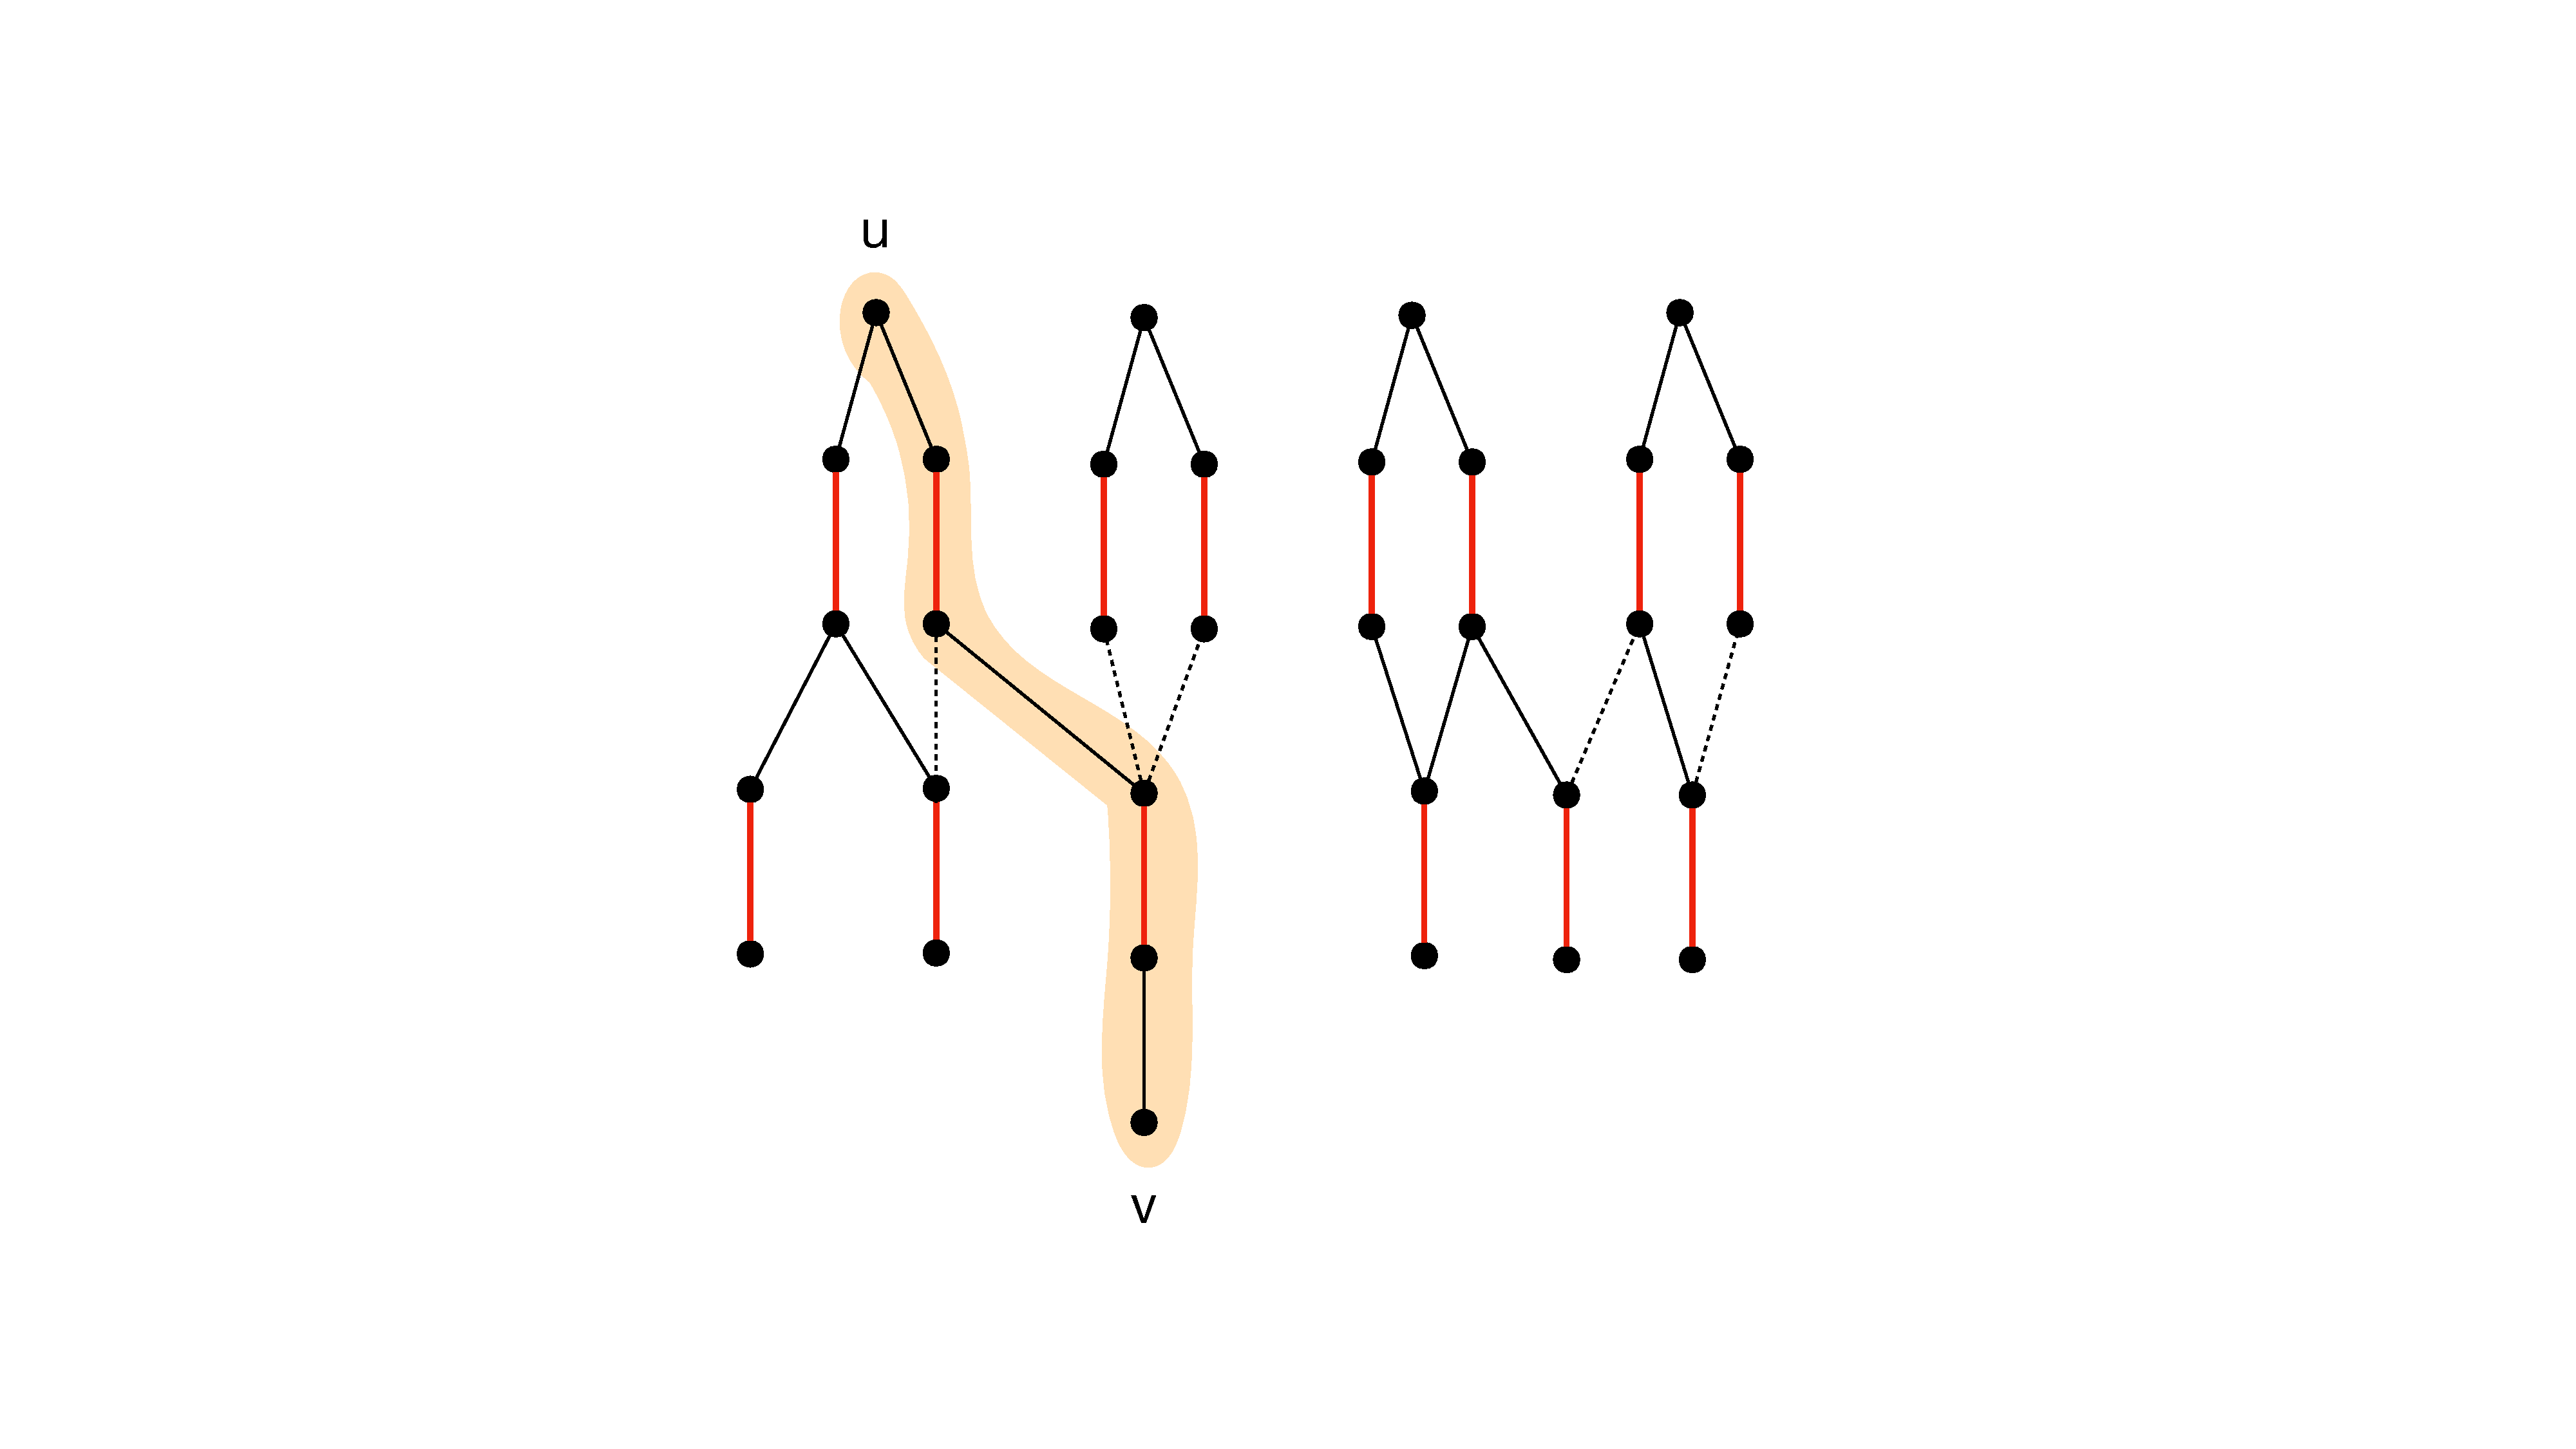
\includegraphics[width=0.5\textwidth]{fig/lecture_matching_bipartite}
	\caption{This picture shows an example of breath-first trees of alternating paths. The vertices on the top level are free vertices in $L$. All solid edges are tree edges, and red edges are matching edges in $M$, and the dashed edges are non-tree edges in $E\setminus M$. The orange path highlights an augmenting path found by the search tree.}
	\label{fig:bipartite}
\end{figure}

%\mprobst{This paragraph should be broken down and there should be a definition explaining the terms 'free vertex' and 'alternating paths'. BFS from free vertices might already confuse students, so maybe introduce a dummy source?  I feel if you just outline a full proof that it works in unweighted, and have pseudo-code that looks like Ford-Fulkerson, then you can teach it in 10 mins and people are less confused and have a better basis. It is quite non-trivial to see this tbh.}

\subsection{General Edge Weights}
However, the above scheme does not work directly with edge weights. To handle general edge weights, we use a technique called the primal-dual method. The bipartite maximum weight matching problem can be formalized as an integer linear program: %\mprobst{Use $\xx$ and $\yy$ for consistent vecotr notation. You could also use more compact notation, like $\xx^T \vecone \leq 1, \max_{\xx} \wts^T \xx, \BB \yy \geq \ww$, etc. if you want to, that would match previous chapters. But using your notation is also fine of course}
$$\begin{aligned}
	&\max \sum_{e\in E}\wts(e)\cdot x(e)\\
	s.t.\quad & x(e)\in \{0, 1\}	&	\forall e\in E\\
	& \sum_{e\ni u}x(e) \leq 1	&	\forall u\in V
\end{aligned}$$

Relax the constraint $x(e)\in \{0, 1\}$ to $x(e)\in [0, 1]$ and write the dual program:
$$\begin{aligned}
	&\min \sum_{u\in V}y(u)\\
	s.t.\quad &	y(u) + y(v)\geq \wts(e)	&\forall e = (u, v)\in E\\
	&	y(u)\geq 0	&\forall u\in V
\end{aligned}$$

The basic strategy is to repeatedly augment a feasible primal integral solution $\{x(e)\mid e\in E\}$, which is actually a matching $M$, as well as a feasible dual solution $\{y(u)\mid u\in V\}$ and in the end reach the condition that:
$$\sum_{e\in E}\wts(e)\cdot x(e) = \sum_{u\in V}y(u)$$
By the weak duality of linear programs, we conclude that the our matching $M$ should be optimal at the end.

To describe the algorithm, we rely on the notation of tightness.
\begin{definition}
	An edge $e = (u, v)$ is \textbf{tight} if $y(u) + y(v) = \wts(e)$.
\end{definition}
At the beginning of the algorithm, set $M = \emptyset$, $y(u) = W,\forall u\in L$ and $y(v) = 0, \forall v\in R$, so $y$ would be a feasible solution for the dual program. During the augmentation steps, define $G_y = (L\cup R, E_y)$ to be the subgraph of $G$ consisting of all tight edges. Throughout the algorithm, we will maintain the following invariant.

% \mprobst{For black board teaching, pseudo-code would be nicer.}
\begin{invariant}\label{match-tight}
	During the algorithm, all edges in $M$ are tight. Furthermore, for any $u\in L\setminus V(M)$, we have $y(u) = \min_{v\in L}\{y(v)\}$.
\end{invariant}
In each round, the algorithm augment $M$ in $G_y$ as long as it could, and then adjust the vertex labels $y$ so that more edges become tight. The algorithm terminates when $y(v) = 0$ for all free vertex $v$.

\begin{algorithm}
	\caption{maximum weight matching in graph $G = (L\cup R, E, \wts)$}\label{hungarian}
	initialize $M \leftarrow \emptyset$, $y(u) \leftarrow W, y(v)\leftarrow 0, \forall u\in L, v\in R$\;
	\While{$y(u)>0$ for some $u\notin V(M)$}{
		define $G_y = (L\cup R, E_y)$ to be the subgraph of all tight edges\;
		repeatedly augment $M$ in graph $G_y$, until there is no more augmenting paths in the same way as \Cref{bipartite-mcm}\;
		\tcc{adjust the dual variables $y$ to make more tight edges}
		assign directions to edges in $G_y$\;
		compute $Z\subseteq V$ which is the set of vertices reachable from all free vertices in $L$ in directed graph $\overrightarrow{G_y}$\;
		define $F = \{(u, v)\in E\setminus E_y\mid u\in L\cap Z, v\in R\setminus Z\}$ and $\Delta = \min\left\{\min_{(u, v)\in F}\{y(u) + y(v) - \wts(u, v), \min_{u\in L}\{y(u)\}\right\}$\;
		update $y(u)\leftarrow y(u) - \Delta, y(v)\leftarrow y(v) + \Delta, \forall u\in L\cap Z, v\in R\cap Z$\;
	}
	\Return $M$\;
\end{algorithm}

The advantage of finding augmenting paths in graph $G_y$ is that it preserves Invariant \ref{match-tight} because by definition all edges in $G_y$ are tight. The main question here is how to adjust the dual variables to generate more tight edges.

To do this, we will implement dual adjustment through a reachability problem in graph $G_y$. For any edge $(u, v)\in (L\times R)\cap E_y$, if $(u, v)\in M$, assign an edge direction from $v$ to $u$; if $(u, v)\notin M$, assign an edge direction from $u$ to $v$. Call this directed graph $\overrightarrow{G_y}$. Compute a vertex subset $Z\subseteq V$ which is the set of vertices reachable from all free vertices in $L$. Define an edge set $F\subseteq E\setminus E_y$ as well as a value $\Delta$:
$$F = \{(u, v)\in E\setminus E_y\mid u\in L\cap Z, v\in R\setminus Z\}$$
$$\Delta = \min\left\{\min_{(u, v)\in F}\{y(u) + y(v) - \wts(u, v), \min_{u\in L}\{y(u)\}\right\}$$
Then, for each $u\in L\cap Z$ decrease $y(u)\leftarrow y(u) - \Delta$, and for each $v\in R\cap Z$ increase $y(v)\leftarrow y(v) + \Delta$. After this dual adjustment, more tight edges will appear. Check \Cref{fig:dual} for an illustration.

\begin{figure}
	\centering
	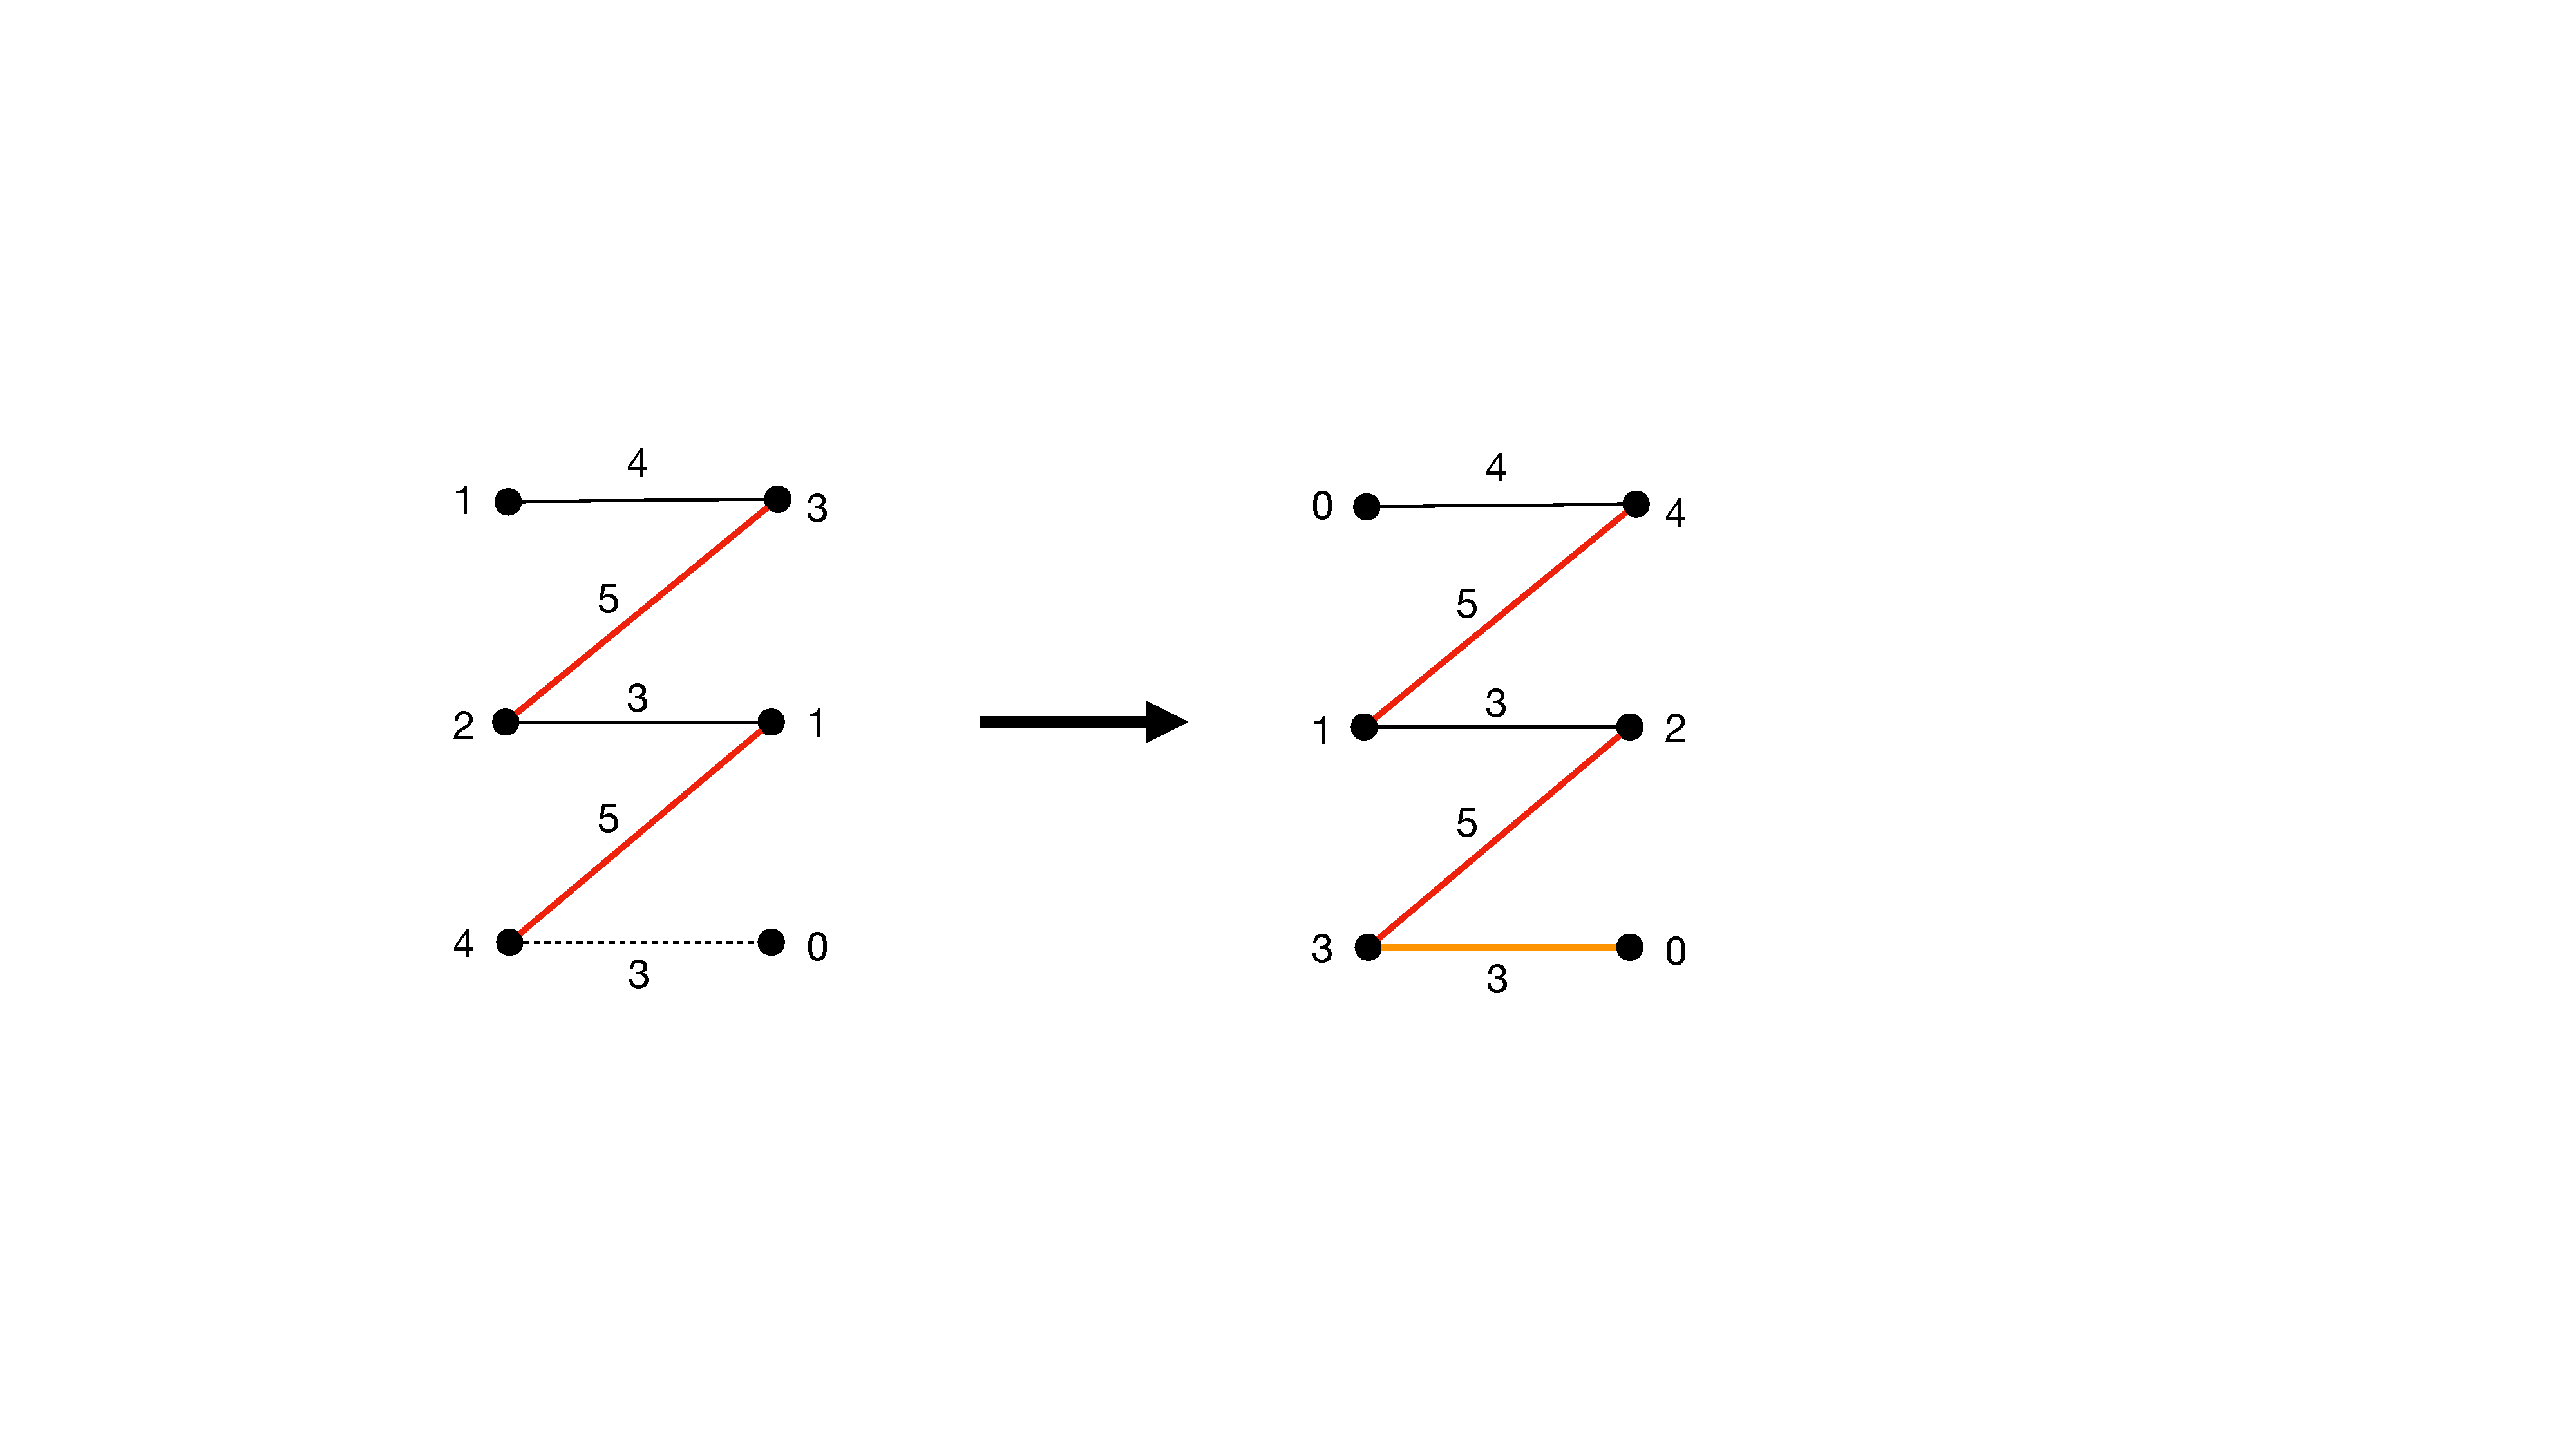
\includegraphics[width=10cm]{fig/lecture_matching_dual}
	\caption{In the example, solid edges are tight, and red edges are matched. Before the dual adjustment, the dashed edge on the left-hand side is not tight. After the dual adjustment, the orange edge is a new tight edge.}
	\label{fig:dual}
\end{figure}

The pseudo-code \Cref{hungarian} summarizes this algorithm.

\begin{observation}
	Invariant \ref{match-tight} is preserved by dual adjustments, and $E_y$ is only monotonically growing.
\end{observation}

\begin{lemma}
	The runtime of the algorithm is $O(m^2)$.
\end{lemma}
\begin{proof}
	Each iteration can be implemented in $O(m)$ which mainly computes reachability in the directed version of $G_y$. In each iteration of the while-loop, if $\Delta > \min_{u\in L}\{y(u)\}$, then $\Delta$ would be equal to some $y(u_*) + y(v_*) - \wts(u_*, v_*), (u_*, v_*)\in F$, after adjusting the dual variables, $G_y$ would now include a new edge $(u_*, v_*)$. Otherwise, if $\Delta = \min_{u\in L}\{y(u)\}$, all free vertices may now have zero labels, so the algorithm terminates. Overall, there can be at most $m$ iterations, so the runtime is $O(m^2)$. Note that a tight edge $(u, v)$ never becomes non-tight again because the decrease of $y(u)$ cancels out with the increase of $y(v)$ due to the way we adjust the vertex labels.
\end{proof}

\begin{lemma}
	When the algorithm terminates, $M$ is a maximum weight matching.
\end{lemma}
\begin{proof}
	Let $M^\star$ be the a maximum weight matching. Let us show that $\wts(M)\geq \wts(M^\star)$. In fact, since all edges in $M$ are tight and free vertices have zero labels, we have:
	$$\begin{aligned}
		\wts(M) &= \sum_{u\in V}y(u)\\
				&= \sum_{(u, v)\in M^\star}(y(u) + y(v)) + \sum_{u\notin V(M^\star)}y(u)\\
				&\geq \sum_{(u, v)\in M^\star} \wts(u, v) = \wts(M^\star)\qedhere
	\end{aligned}$$
\end{proof}

\subsection{Faster Implementation}
Next, we show how to optimize the runtime from $O(m^2)$ to $\tilde{O}(mn)$. Notice that $M$ could be augmented by at most $n$ times, while the graph $G_y$ may grow for at most $m$ times. So the bottleneck of the algorithm is growing $G_y$, and most of the $m$ while-loop iterations are about growing $G_y$, not augmenting $M$. So, to improve the runtime, the idea is to compress multiple consecutive while-loop iterations which only enlarge $G_y$ into a single iteration, such that the next iteration can augment $M$.

To implement this idea, the main observation is that the concatenation of multiple while-loop iterations is actually a shortest path computation from left free vertices to right free vertices. More specifically, for each edge $(u, v)\in E$, assign edge length $\mu(u, v) = y(u) + y(v) - \wts(u, v)\geq 0$, and orient all matching edges from $R$ to $L$, and non-matching edges from $L$ to $R$. Then, add a terminal $s$ which is connected to all free vertices in $L$ (with zero weight edges). Call this directed weighted graph $\overrightarrow{H_y} = (V, E, \mu)$. After that, compute the single-source shortest paths from $s$ in $\overrightarrow{H_y}$.

Let $t\in R\cap V(M)$ be the free vertex which minimizes $d(s, t, \overrightarrow{H_y})$, and define: $$\Delta = \min_{u\in L}\left\{d(s, t, \overrightarrow{H_y}), y(u)\right\}$$
Then, for each $u\in L$ such that $d(s, u, \overrightarrow{H_y})\leq \Delta$, update the vertex label: $$y(u)\leftarrow y(u) - \Delta + d(s, u, \overrightarrow{H_y})$$
and for each $v\in R$ such that $d(s, v, \overrightarrow{H_y})\leq \Delta$, update the vertex label:
$$y(v)\leftarrow y(v) + \Delta - d(s, v, \overrightarrow{H_y})$$
This algorithm is summarized in \Cref{fast-hung}.

\begin{algorithm}
	\caption{faster maximum weight matching in graph $G = (L\cup R, E, \wts)$}\label{fast-hung}
	initialize $M \leftarrow \emptyset$, $y(u) \leftarrow W, y(v)\leftarrow 0, \forall u\in L, v\in R$\;
	\While{$y(u)>0$ for some $u\notin V(M)$}{
		repeatedly augment $M$ in graph $G_y$, until there is no more augmenting paths\;
		\tcc{adjust the dual variables $y$ to make more tight edges}
		build directed weighted graph $\overrightarrow{H_y}$\;
		let $t\in R\cap V(M)$ be the free vertex which minimizes $d(s, t, \overrightarrow{H_y})$\;
		compute $\Delta \leftarrow \min_{u\in L}\left\{d(s, t, \overrightarrow{H_y}), y(u)\right\}$\;
		\For{$u\in L$ such that $d(s, u, \overrightarrow{H_y})\leq \Delta$}{
			update the vertex label $y(u)\leftarrow y(u) - \Delta + d(s, u, \overrightarrow{H_y})$\;
		}
		\For{$v\in R$ such that $d(s, v, \overrightarrow{H_y})\leq \Delta$}{
			update the vertex label $y(v)\leftarrow y(v) + \Delta - d(s, v, \overrightarrow{H_y})$\;
		}
	}
	\Return $M$\;
\end{algorithm}

First, let us verify that our dual adjustment scheme preserves feasibility of the dual solution as well as Invariant \ref{match-tight}.

\begin{lemma}
	In each iteration of the while-loop, dual feasibility and Invariant \ref{match-tight} are both preserved by our dual adjustment scheme.
\end{lemma}
\begin{proof}
	Let use $y$ and $y'$ to denote the dual variables before and after the adjustment, respectively. First, we verify that all $y'$ values are non-negative. In fact, for any $v\in R$ such that $d(s, v, \overrightarrow{H_y}) \leq \Delta$, we have $y'(v) = y(v) + \Delta - d(s, v, \overrightarrow{H_y})\geq 0$; for any $u\in L$, by definition of $\Delta$, we know that $\Delta \leq y(u)$, and therefore $y'(u) = y(u) - \Delta + d(s, u, \overrightarrow{H_y})\geq 0$.
	
	Now, consider any edge $(u, v)\in E\cap (L\times R)$. Previously before the change, we had $y(u) + y(v) - \wts(u, v) = \mu(u, v) \geq 0$. Since $y'(v)$ does not decrease, we only need to worry about the case when $y'(u) < y(u)$. There are two cases.
	
	\begin{itemize}
		\item $(u, v)\notin M$. In this case, noticing that we always have $y'(v) \geq y(v) + \Delta - d(s, v, \overrightarrow{H_y})$, therefore
		$$\begin{aligned}
			y'(u) + y'(v) &\geq y(u) + y(v) + d(s, u, \overrightarrow{H_y}) - d(s, v, \overrightarrow{H_y})\\
			&= \wts(u, v) + \mu(u, v) +d(s, u, \overrightarrow{H_y}) - d(s, v, \overrightarrow{H_y})\\
			&\geq \wts(u, v)
		\end{aligned}$$
		
		\item $(u, v)\in M$. In this case, $(u, v)$ is the only in-edge for $u$, and so $d(s, u, \overrightarrow{H_y}) = d(s, v, \overrightarrow{H_y})$. Therefore, 
		$$\begin{aligned}
			y'(u) + y'(v) &= y(u) + y(v) + d(s, u, \overrightarrow{H_y}) - d(s, v, \overrightarrow{H_y})\\
			&= \wts(u, v) +d(s, u, \overrightarrow{H_y}) - d(s, v, \overrightarrow{H_y})\\
			&= \wts(u, v)
		\end{aligned}$$
		This equality also proves that all matching edges in $M$ remain tight after the dual adjustment.
	\end{itemize}
	Finally, for Invariant \ref{match-tight}, notice that $d(s, u , \overrightarrow{H_y}) = 0$ for all free vertices $u\in L$, the vertex labels of free vertices on $L$ have decreased by the same amount $\Delta$. So Invariant \ref{match-tight} also holds.
\end{proof}

Next, let us argue that after the dual adjustment, a new augmenting path shows up in $G_y$.

\begin{lemma}
	In each iteration of the while-loop, after the dual adjustment, either a new augmenting path in $G_y$ shows up, or the algorithm terminates.
\end{lemma}
\begin{proof}
	If $\Delta = \min_{u\in L}\{y(u)\}$, then after the dual adjustment, all the free vertices have zero vertex labels, so the algorithm would terminate. Otherwise, $\Delta =  d(s, t, \overrightarrow{H_y})$.
	
	Let $P$ be the shortest path from $s$ to $t$ in graph $\overrightarrow{H_y}$. We claim that all edges on $P$ become tight after the dual adjustment, which would imply that $G_y$ may now contain a new augmenting path. In fact, for any edge $(u, v)\in P$, if $u\in L, v\in R$, then 
	$$\begin{aligned}
		y'(u) + y'(v) &= y(u) + y(v) + d(s, u, \overrightarrow{H_y}) - d(s, v, \overrightarrow{H_y})\\
		&= \wts(u, v) + \mu(u, v) + d(s, u, \overrightarrow{H_y}) - d(s, v, \overrightarrow{H_y}) \\
		&=\wts(u, v)
	\end{aligned}$$
	The last inequality holds as $P$ is the shortest path and thus $\mu(u, v) + d(s, u, \overrightarrow{H_y}) = d(s, v, \overrightarrow{H_y})$. Otherwise, if $u\in R, v\in L$, then $(u, v)\in M$, and therefore
	$$\begin{aligned}
		y'(u) + y'(v) &= y(u) + y(v) + d(s, u, \overrightarrow{H_y}) - d(s, v, \overrightarrow{H_y})\\
		&= \wts(u, v) +d(s, u, \overrightarrow{H_y}) - d(s, v, \overrightarrow{H_y})\\
		&= \wts(u, v)
	\end{aligned}$$
	This concludes the proof.
\end{proof}

By the above statement, we know that the while-loop contains at most $n$ iterations, and so the total runtime becomes $\tilde{O}(mn)$ if we use Dijkstra's algorithm to compute single-source shortest path in each iteration.

\section{General Graph Matching}

\subsection{Unit Edge Weights}

Let us now turn to maximum matching in general graphs. The main technical difficulty with general graphs is that we cannot formulate augmenting paths as a reachability problem (even in unit-weight graphs) as we did in bipartite graphs due to odd cycles formed by alternating paths. This technical issue was addressed by Edmonds \cite{edmonds1965paths}. The key notion of Edmonds' algorithm is called \emph{blossom}. Roughly speaking, given a matching $M$, a blossom is an odd-length alternating cycle whose constituents are vertices or smaller blossoms. More formally, a blossom is specified by a tuple $(B, E_B, \beta(B))$, where $B\subseteq V$ is a vertex subset, $E_B\subseteq E$ is an edge subset, $\beta(B)\in B$ is a special vertex called the \emph{base}. Blossoms follow an inductive definition below.

\begin{definition}[\cite{edmonds1965paths}]
A single vertex $v$ forms a trivial blossom as a tuple $(\{v\}, \emptyset, v)$. Inductively, let $B_1, B_2, \ldots, B_{2l+1}$ be an odd sequence of blossoms. Suppose there exists a sequence of edges $e_1, e_2, \ldots, e_{2l+1}$ such that $e_i\in B_i\times B_{i+1}$ ($B_{2l+2} = B_1$). The tuple $\left(\bigcup_{i=1}^{2l+1}B_i, \bigcup_{i=1}^{2l+1}E_{B_i}, \beta(B_1)\right)$ is identified as a blossom if $e_i\in M$ iff $i$ is even. Check \Cref{fig:blossom} for an illustration.
\end{definition}

% \mprobst{This is a bit confusing... isn't there an easier definition that is more intuitive? Maybe in some Goemanns lecture notes?}

\begin{figure}
	\centering
	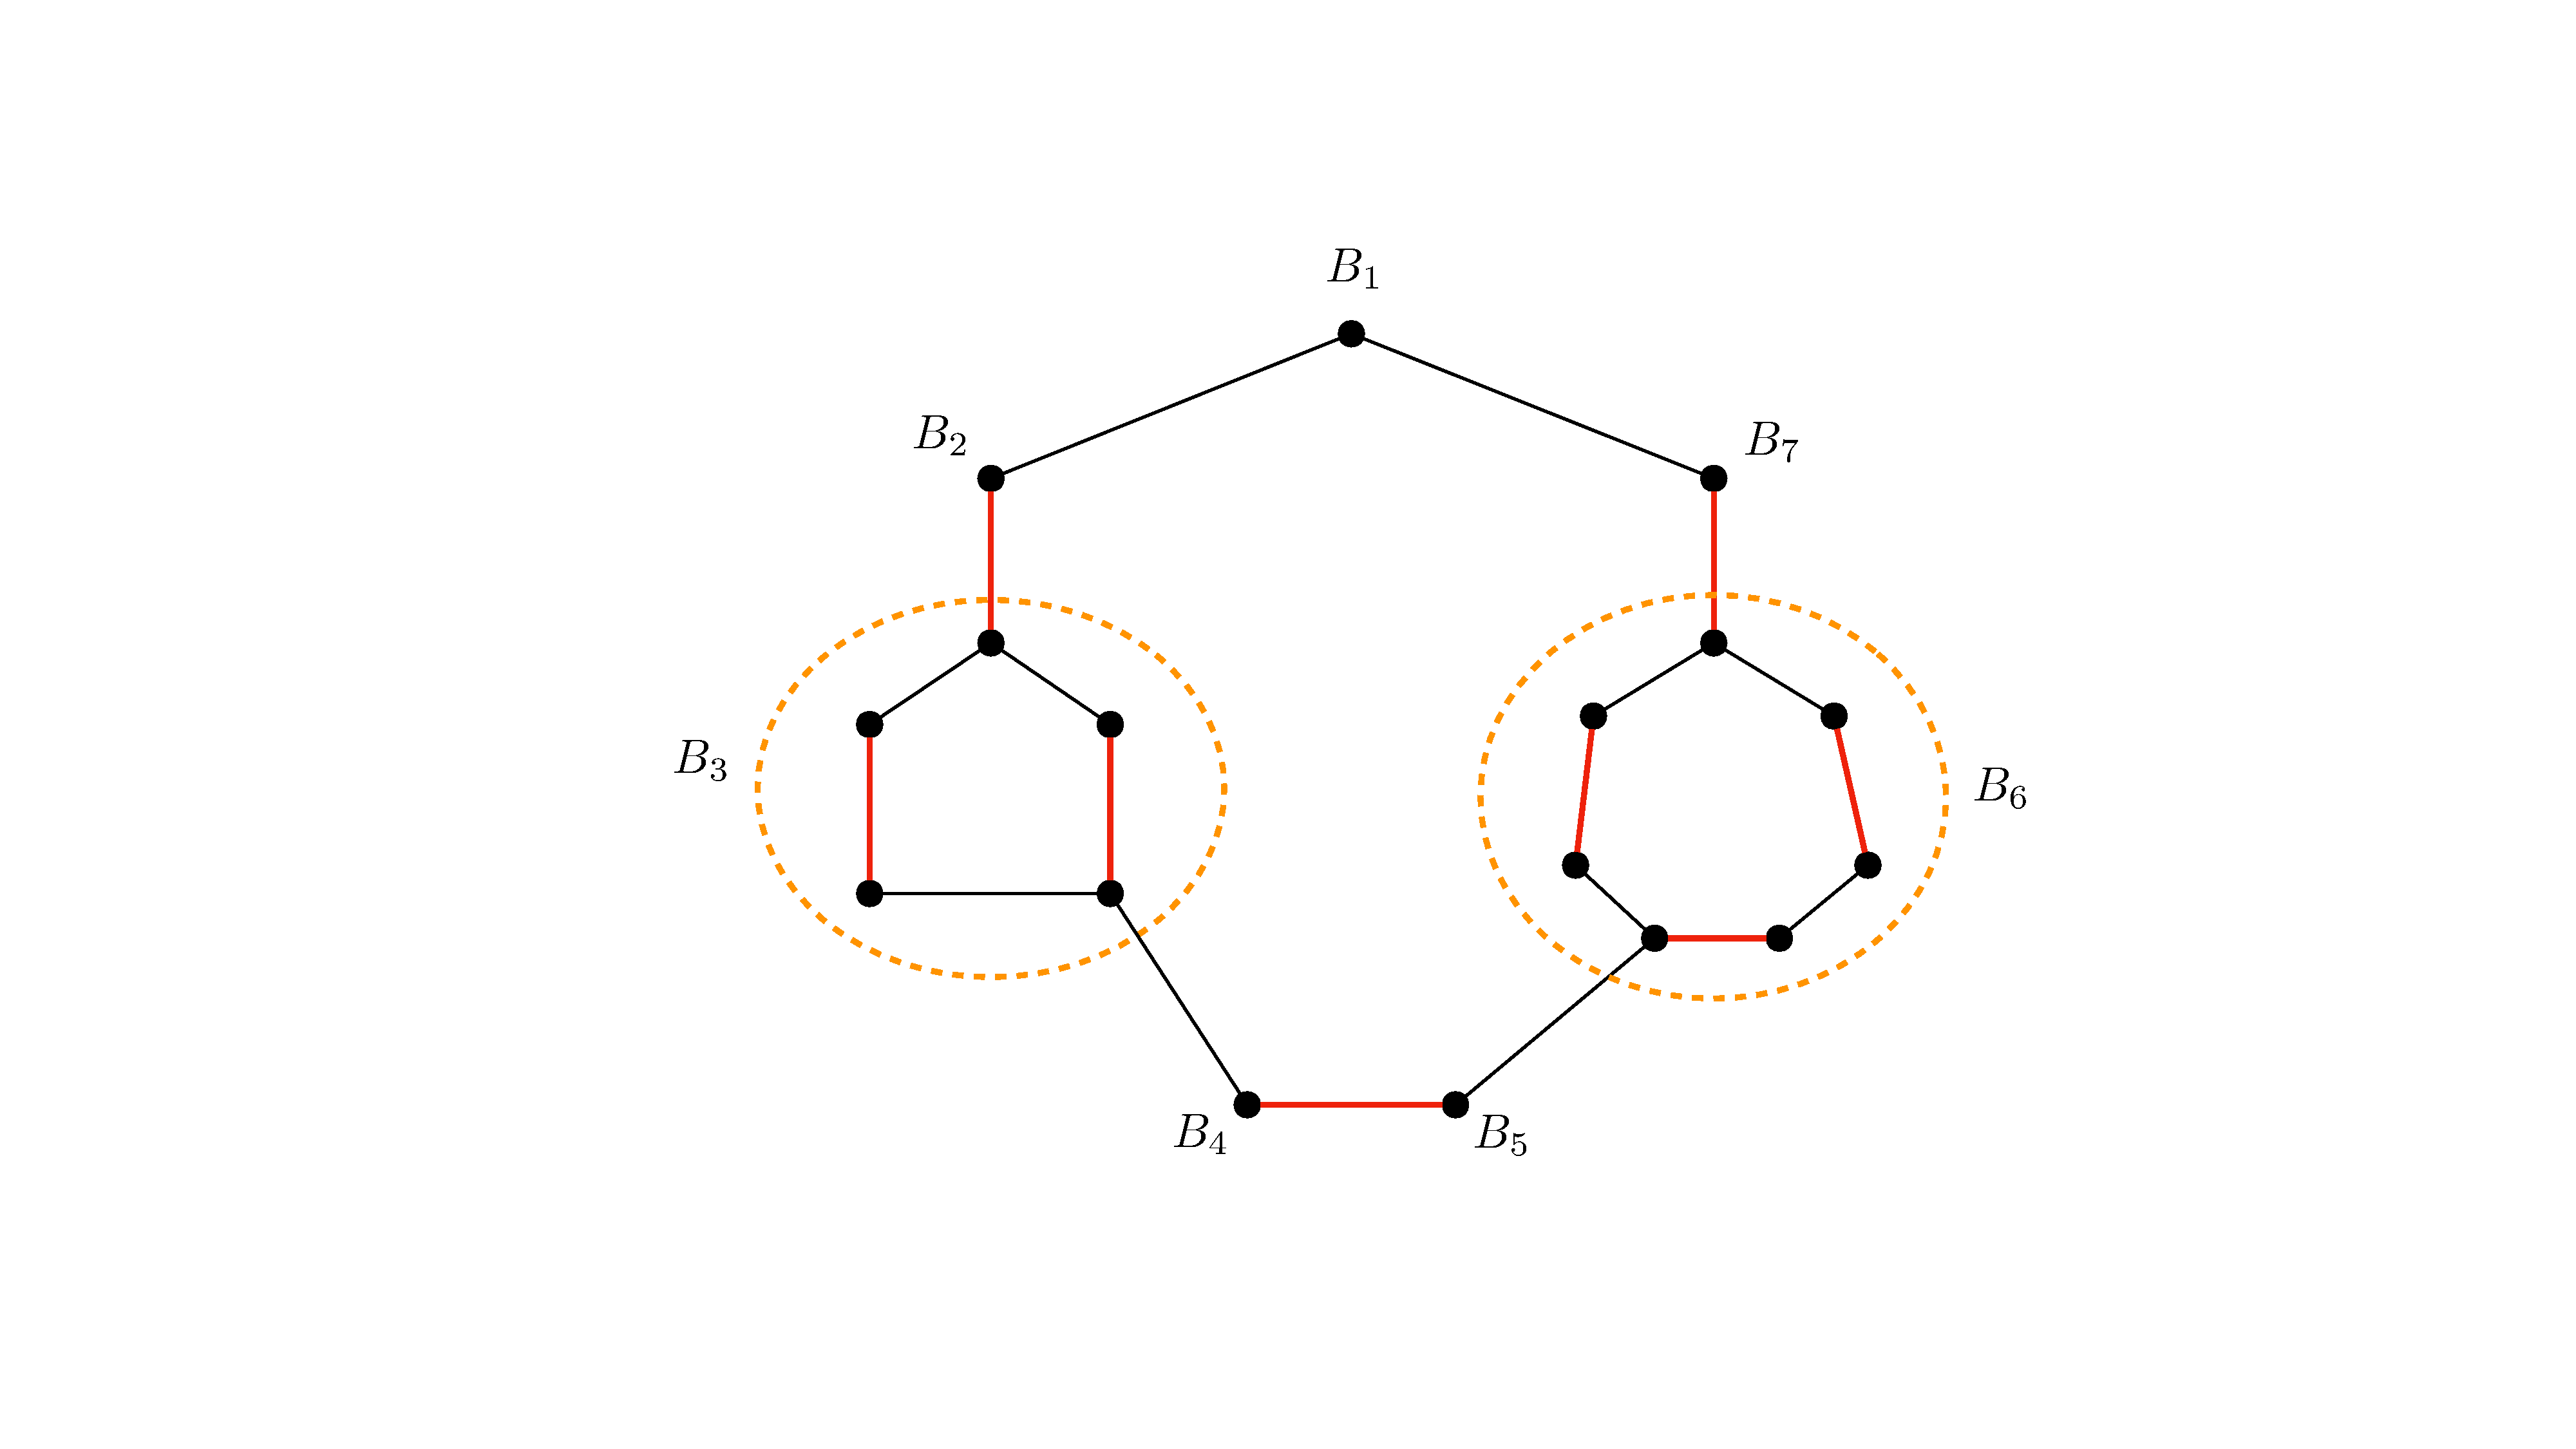
\includegraphics[width=10cm]{fig/lecture_matching_blossom}
	\caption{This picture shows an example of a blossom, where the red edges are matching edges, and the black ones are non-matching edges. The two subgraphs in the dashed orange cycles are two smaller blossoms.}
	\label{fig:blossom}
\end{figure}

We can show that for any blossom $(B, E_B, \beta(B))$, $E_B\cap M$ matches all vertices in $B$ but $\beta(B)$. The key property of blossoms is the following statement.
\begin{observation}
	If the base of a blossom is is free, then all vertices in the blossom are also reachable from this free base vertex via simple alternating paths.
\end{observation}
This property implies that we can shrink a blossom into a single node if this blossom is reachable from free vertices. Informally speaking, to search for augmenting paths from free vertices, we can apply the same breath-first search through alternating paths. If we encounter some odd cycles during the process, then this odd cycle must form a blossom. In this case, we can shrink the entire blossom into a single node, and then continue on with the breath-first search procedure. As the graph cannot shrink indefinitely, we will find an augmenting path at the end in polynomial time.

To formalize this idea, we will maintain a laminar family of blossoms $\Omega\subseteq 2^V$. For each free vertex $u\in V$, we will maintain a tree $T_u$ rooted at $u$ in the contracted graph $\mathcal{G} = G / \Omega$ where each the blossom is contracted into a single node.

\begin{definition}[out/in labels]
	For each node in tree $T_u$, if its distance to the root is even, label this node as \emph{out}, and otherwise label it as \emph{in}. All vertices contracted within blossoms are labeled out or in accordingly.
\end{definition}

The trees $\{T_u\mid u\notin V(M)\}$ will satisfy the following properties.
\begin{itemize}
	\item All the rooted trees $\{T_u\mid u\notin V(M)\}$ will be vertex-disjoint.
	\item Each root-to-leaf path in any such tree $T_u$ will be an alternating path in $\mathcal{G}$, and each leaf node in $T_u$ is labeled out.
\end{itemize}


To grow all the trees $\{T_u\mid u\notin V(M)\}$, each time we select an arbitrary free vertex $u$ as well as an out vertex $v\in V$ contracted in a leaf node in $B_v\in V(T_u)$. Enumerate all edges $(v, w)\in E$ and consider the following possibilities.
\begin{itemize}
	\item \textbf{Blossom contraction.} Vertex $w$ is residing in a node $B_w\in V(T_u)$. If $w$ is an out vertex, then all the nodes on the tree path between $B_v, B_w$ would make a blossom in $G$; call this blossom $B$, add $B$ to $\Omega$, and contract $B$ in $\mathcal{G}$. Check \Cref{fig:contract} for an illustration.
	
	\begin{figure}
		\centering
		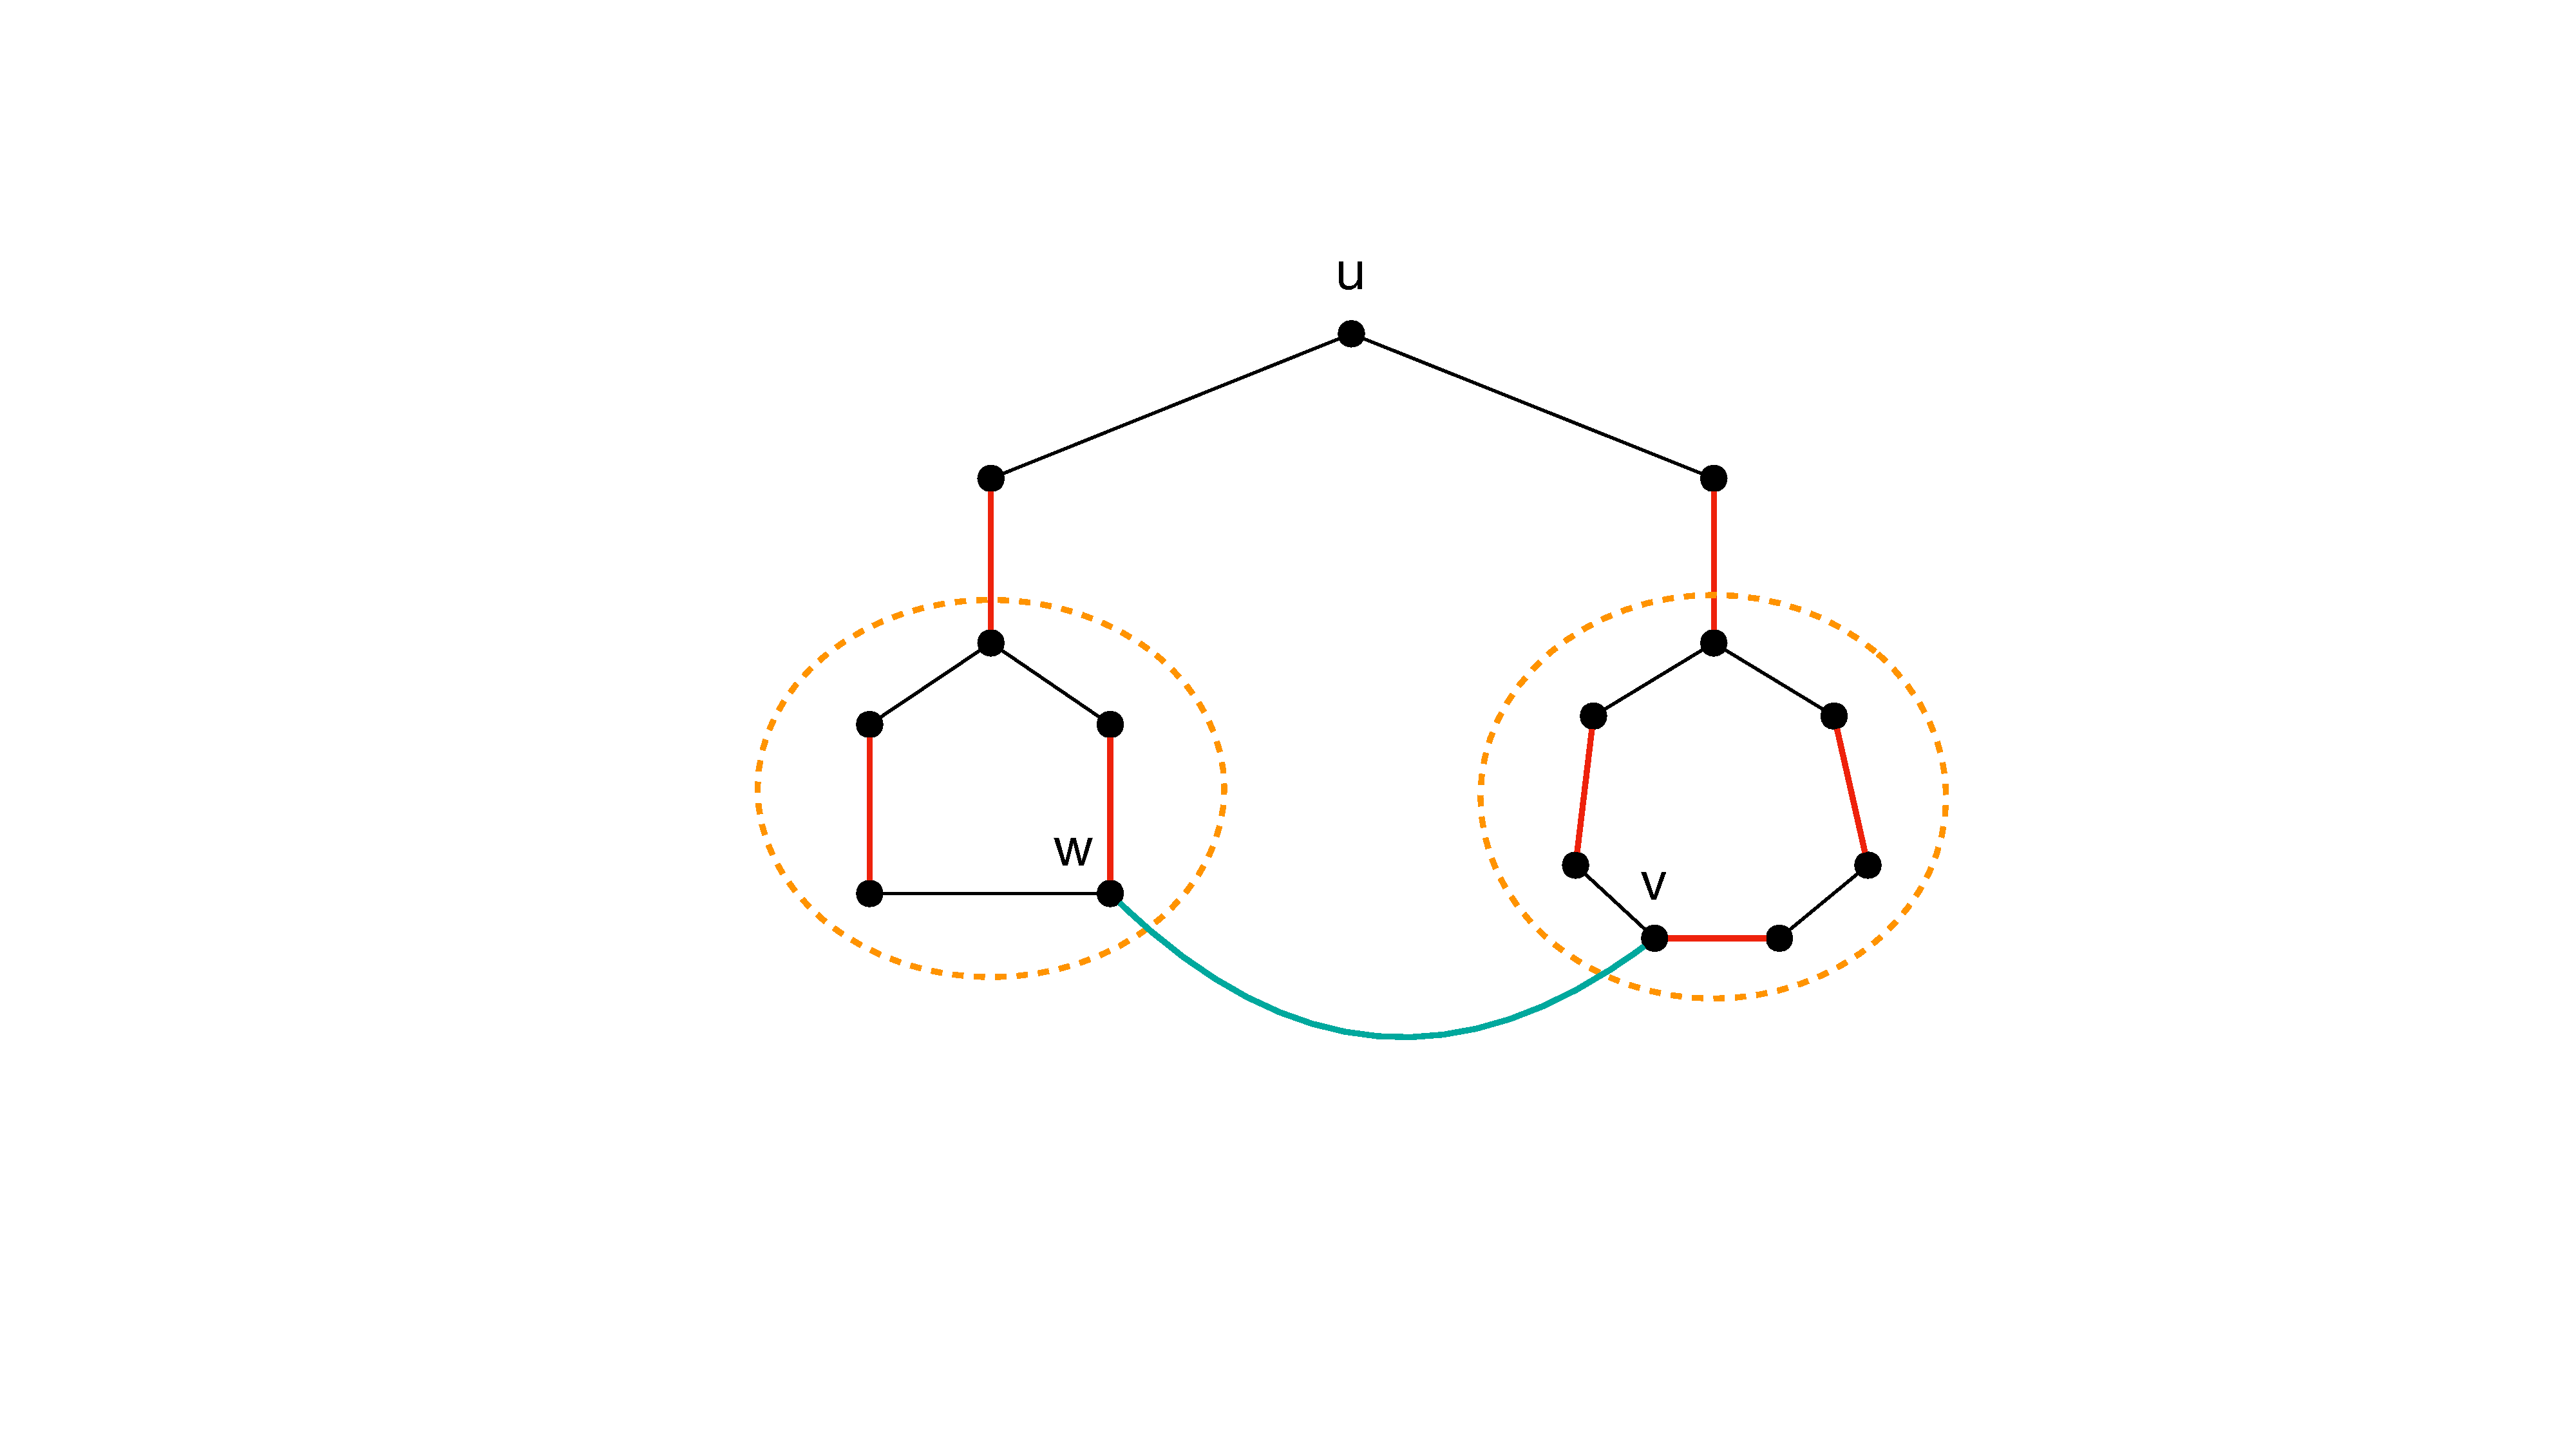
\includegraphics[width=10cm]{fig/lecture_matching_contract}
		\caption{In this picture, all the red and black edges are tree edges of $T_u$, and blue edge $(v, w)$ connects two out vertices. In this example, we can contract the entire tree $T_u$ into a single node.}
		\label{fig:contract}
	\end{figure}
	
	\item \textbf{Tree extension.} Vertex $w$ is currently not in any of the trees $T_{u'}, u'\notin V(M)$. In this case, $w$ cannot be free, and let $(w, z)\in M$ be its matched edge. We argue that $z$ also cannot be in any existing trees $T_{u'}, u'\notin V(M)$, since otherwise $w$ would be added to some trees already. Then, let us add edges both $(v, w), (w, z)$ to tree $T_u$.
	
	\item \textbf{Augmentation.} Vertex $w$ is in another tree $T_{u'}, u'\notin V(M)\setminus \{u\}$. Suppose $w$ is an out vertex, then we have found an augmenting path between $u, u'$. In this case, flip the augmenting path to increase $M$ and start over. Check \Cref{fig:augment} for an illustration.
	
	\begin{figure}
		\centering
		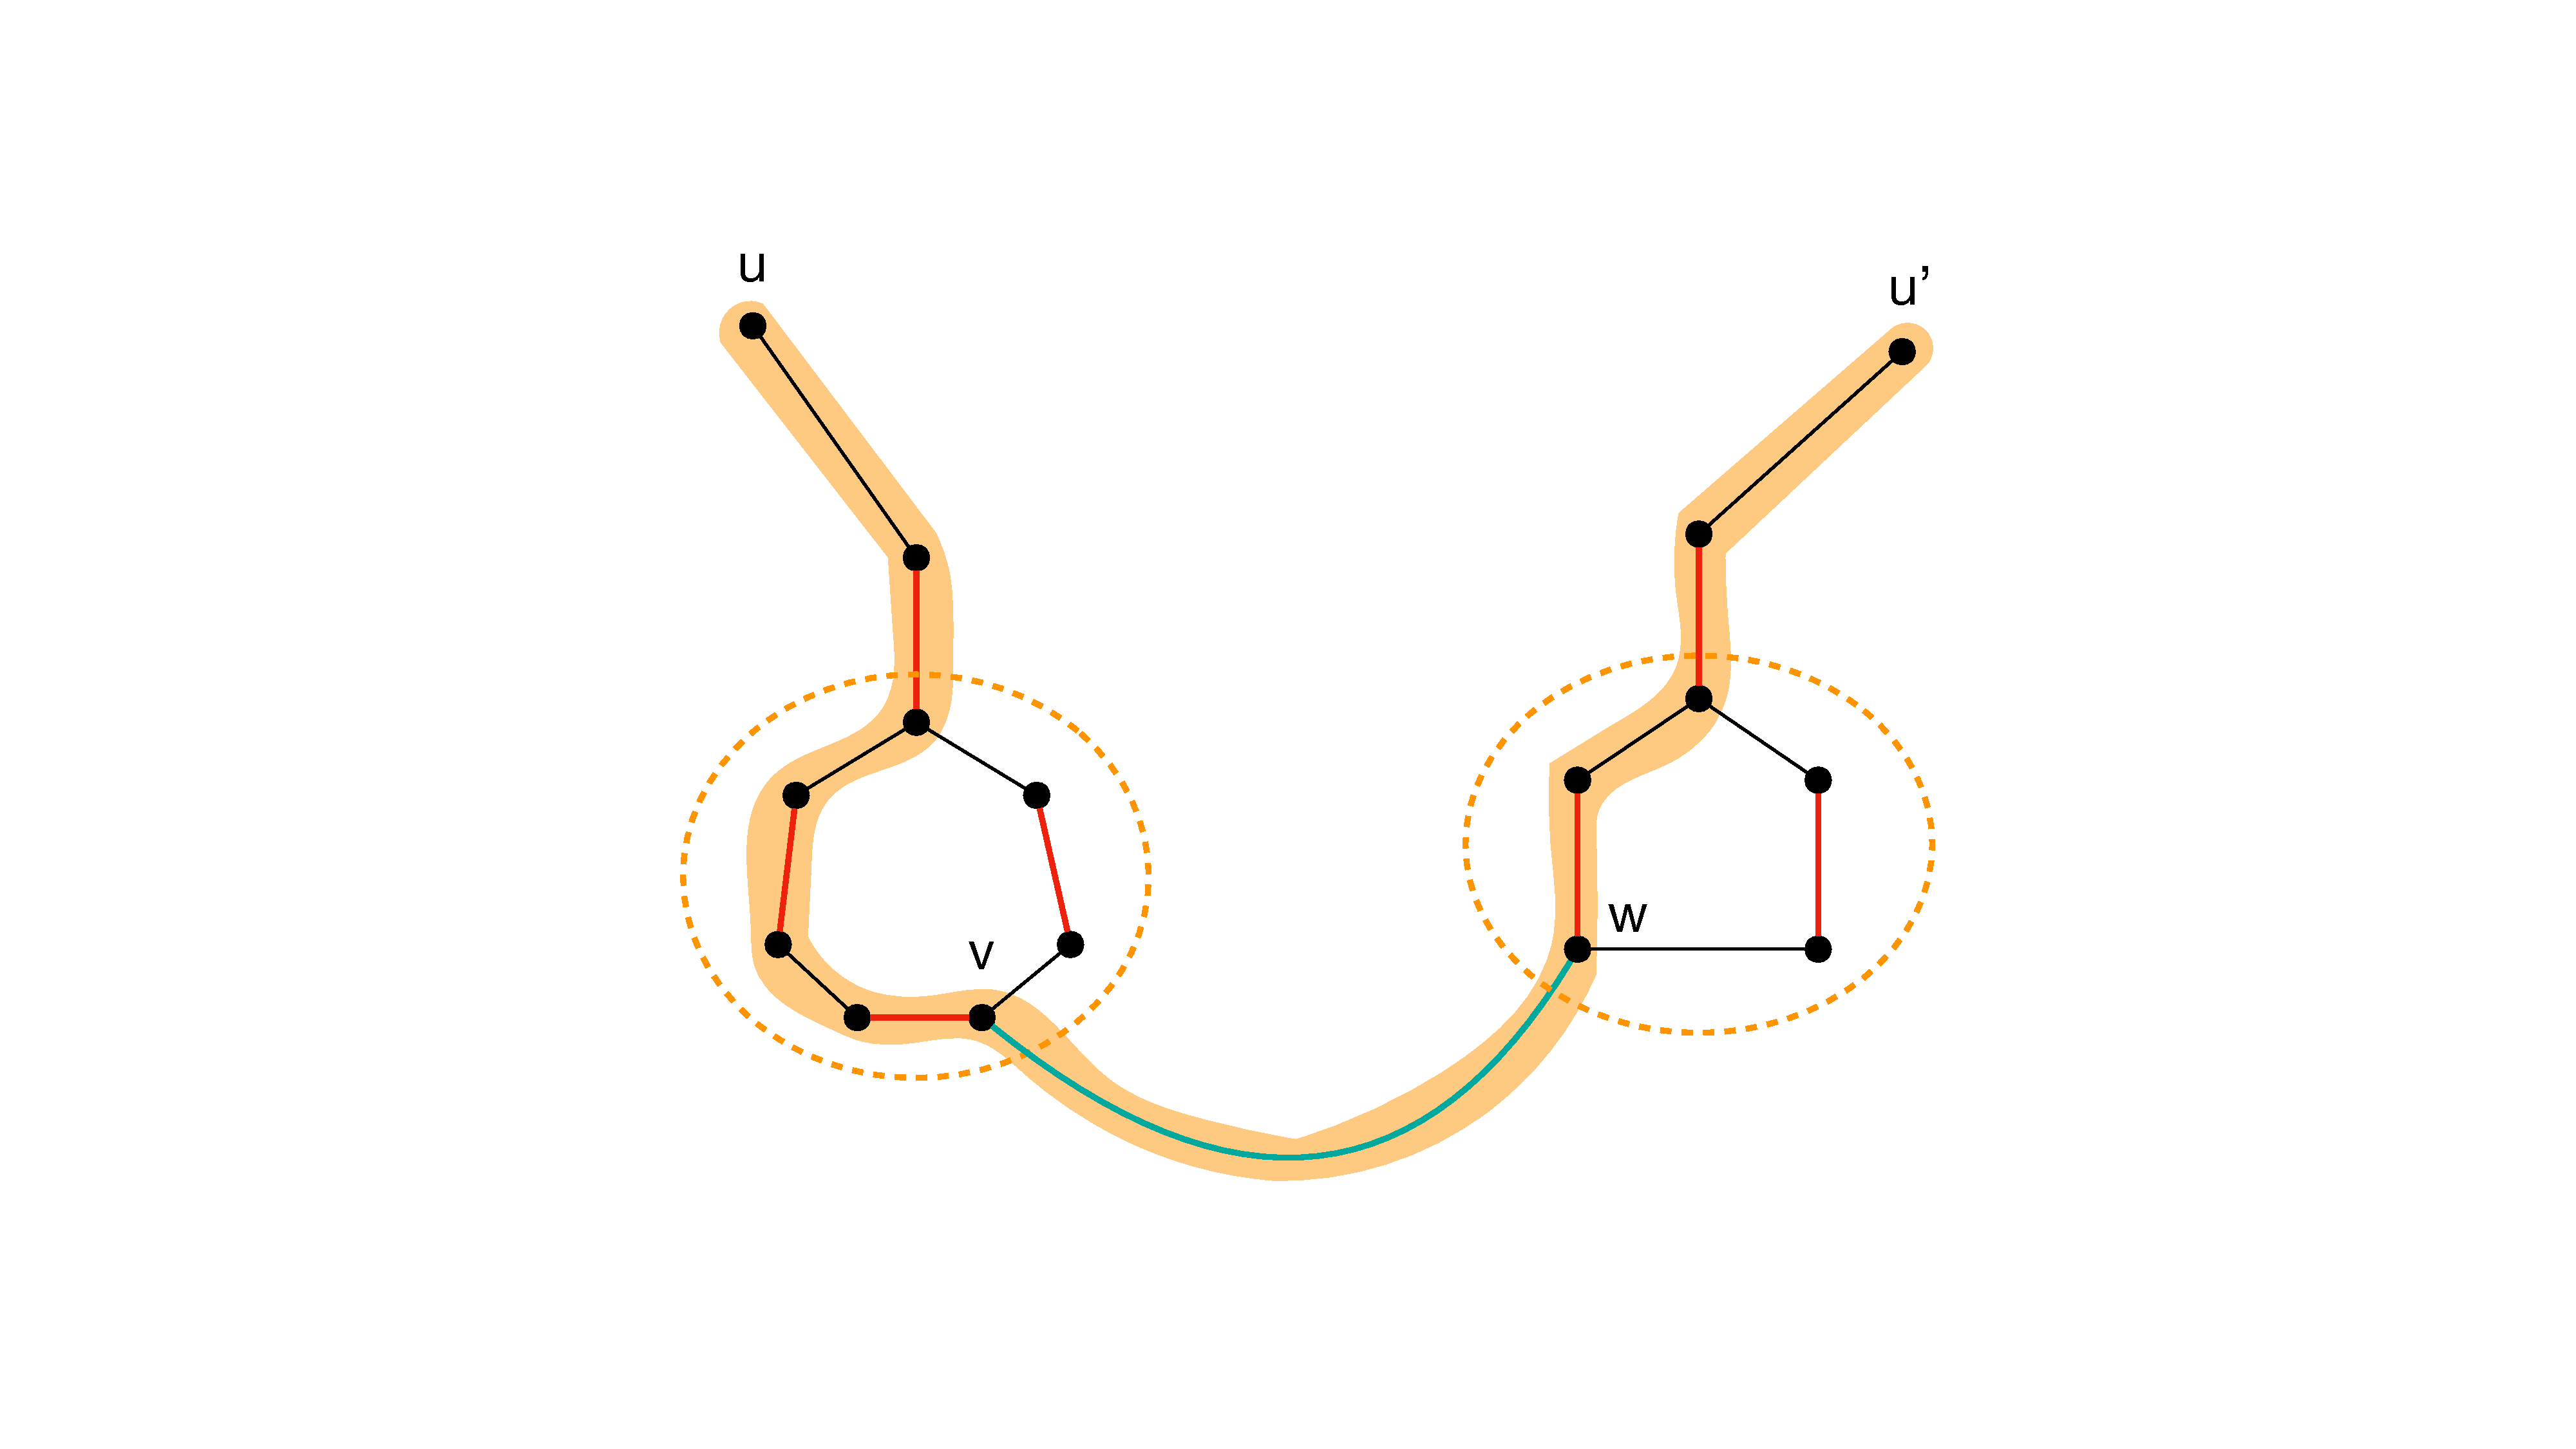
\includegraphics[width=10cm]{fig/lecture_matching_augment}
		\caption{In this picture, all the red and black edges are tree edges of $T_u, T_{u'}$, and the blue edge $(v, w)$ connects two out vertices in $T_u, T_{u'}$. Then, we can find an augmenting path between $u, u'$ which is highlighted as the orange path.}
		\label{fig:augment}
	\end{figure}
\end{itemize}




The above algorithm is summarized as pseudo-code \Cref{alg:general-mcm}.
\begin{lemma}
	When $M$ is not a maximum matching, then the algorithm always finds an augmenting path.
\end{lemma}
\begin{proof}[Proof sketch]
	Take the maximum matching $M^\star$ and show that in any augmenting path in $M\Delta M^\star$ there should be an edge connecting two out vertices in two different trees $T_u, T_{u'}$.
\end{proof}

\begin{algorithm}
	\caption{maximum matching in general graph $G = (V, E)$}
	\label{alg:general-mcm}
	initialize $M\leftarrow \emptyset$\;
	\Repeat{
		initialize $\Omega\leftarrow \emptyset$, $T_u\leftarrow \{u\}, \forall u\notin V(M)$\;
		\Repeat{
			\For{$u\notin V(M)$, out vertex $v$ contracted in a leaf node $B_v\in V(T_u)$, and $(v, w)\in E$}{
				\If{$w$ is an out vertex}{
					contract all the nodes on the tree path between $B_v, B_w$ as a blossom\;
				}\ElseIf{$w$ is not in any tree}{
					let $(w, z)\in M$ be a matching edge, and add $(v, w), (w, z)$ to $T_u$\;
				}\ElseIf{$w$ is in another tree node $T_{u'}$ and $w$ is an out vertex}{
					flip the augmenting path between $u, u'$ to increase $|M|$\;
					\textbf{break}\;
				}
			}
		}
		\If{$M$ was not augmented in this iteration}{
			\textbf{break}\;
		}
	}
	\Return $M$\;
\end{algorithm}

\subsection{General Edge Weights}

To deal with edge weights, we will combine the previous primal-dual approach with the above blossom approach. The primal linear program for maximum weight matching will have extra constraints for every odd vertex set.
$$\begin{aligned}
	&\max \sum_{e\in E}\wts(e)\cdot x(e)\\
	s.t.\quad & x(e)\in [0, 1]	&	\forall e\in E\\
	& \sum_{e\ni u}x(e) \leq 1	&	\forall u\in V\\
	& \sum_{u, v\in B, (u, v)\in E}\wts(u, v)\leq\frac{|B|-1}{2} & \forall B\subseteq V, |B|\text{ is odd}
\end{aligned}$$


As for the dual program, besides the vertex labels $y: V\rightarrow \mathbb{R}$, we will introduce a new set of variables $z: 2^V\rightarrow \mathbb{R}$ defined on all odd vertex subsets. The dual linear program is formalized below:
$$\begin{aligned}
	&\min \sum_{u\in V}y(u) + \sum_{B\subseteq V, |B|\geq 3 \text{ is odd}}z(B)\cdot \frac{|B|-1}{2}\\
	s.t.\quad &	yz(u, v) = y(u) + y(v) + \sum_{B\supset\{u, v\}}z(B)\geq \wts(e)	&\forall e = (u, v)\in E\\
	&	y(u)\geq 0	&\forall u\in V\\
	&  z(B)\geq 0 &\forall B\subseteq V, |B|\text{ is odd}
\end{aligned}$$

The algorithm maintains a matching $M$ as well as vertex labels $y$, and a laminar family of blossoms $\Omega\subseteq 2^V$ as well as their dual values $z(B), B\in \Omega$; the dual values of all other odd sets will be zero. Let $\mathcal{G}$ be the contracted graph where every maximal blossom in $\Omega$ is contracted into a single node, and then we only keep the tight edges of $E$ under dual variables $y, z$ in $\mathcal{G}$.

The following properties will be ensured during the algorithm.
\begin{invariant}\label{blossom-inv}
	For any free vertex $u$, $y(u) = \min_{v\in V}\{y(v)\}$.
	For each blossom edge $e\in E_B$ for some $B\in \Omega$, $e$ is tight, namely $yz(e) = \wts(e)$. Also, for any maximal blossom $B\in \Omega$ (a tree root in the laminar structure of $\Omega$), we have $z(B) > 0$.
\end{invariant}

At the beginning of the algorithm, initialize $M = \emptyset, y= W, \Omega = \emptyset$. More specifically, given any $M$ and duals $y, z$, begin with empty search trees at each free vertex, and initialize $\Omega\leftarrow \emptyset$. For any free  vertex $u\notin V(M)$, we will maintain a tree $T_u$ in $\mathcal{G}$ rooted at the contracted node containing $u$ such that each root-to-leaf path is an alternating path. As with the unit weight setting, we also label the nodes and vertices as out or in.

If there is currently no augmenting path in $\mathcal{G}$, to generate an augmenting path consisting of tight edges, we will repeatedly adjust the dual variables $y, z$ and extend the search trees. More specifically, given a value $\Delta\geq 0$, we perform the following dual adjustments:
\begin{itemize}
	\item $y(v)\leftarrow y(v) - \Delta$ for all out-vertices, and $y(v)\leftarrow y(v) + \Delta$ for all in-vertices;
	\item $z(B)\leftarrow z(B) + 2\Delta$ for all maximal out-blossoms, and $z(B)\leftarrow z(B) - 2\Delta$ for all maximal in-blossoms.
\end{itemize}

\begin{observation}
	The dual adjustments always preserve Invariant \ref{blossom-inv} as well as dual feasibility.
\end{observation}

We will find the smallest value of $\Delta\geq 0$ such that after the above dual adjustments, one of the following events occur.
\begin{itemize}
	\item \textbf{Termination.} All the free vertices have zero vertex labels. In this case, the algorithm terminates and returns $M$ as a maximum weight matching.
	
	\item \textbf{Blossom dissolution.} The dual value $z(B)$ has reached $0$ for some maximal in-blossoms; this operation does not appear in the unit-weight setting. In this case, remove $B$ from $\Omega$. Suppose blossom $B$ was contained in search tree $T_u$ in $\mathcal{G}$, the sub-blossoms of $B$ are connected as an odd alternating cycle $B_1, B_2, \ldots, B_{2k+1}$. As $B$ was an in-blossom, its parent in $B$ must be connected with $B$ via a non-matching edge with one endpoint residing in a sub-blossom $B_i$. Without loss of generality, assume $i$ is an odd integer. Then, add the entire alternating path $B_1, B_2, \ldots, B_i$ to search tree $T_u$, and discard $B_{i+1}, B_{i+2}, \ldots B_{2k+1}$ from $T_u$. After that, label $B_1, B_2, \ldots, B_i$ as in or out-blossoms according to their distance parities to root of $T_u$. Check \Cref{fig:dissolve} for an illustration.
	 
	\begin{figure}
		\centering
		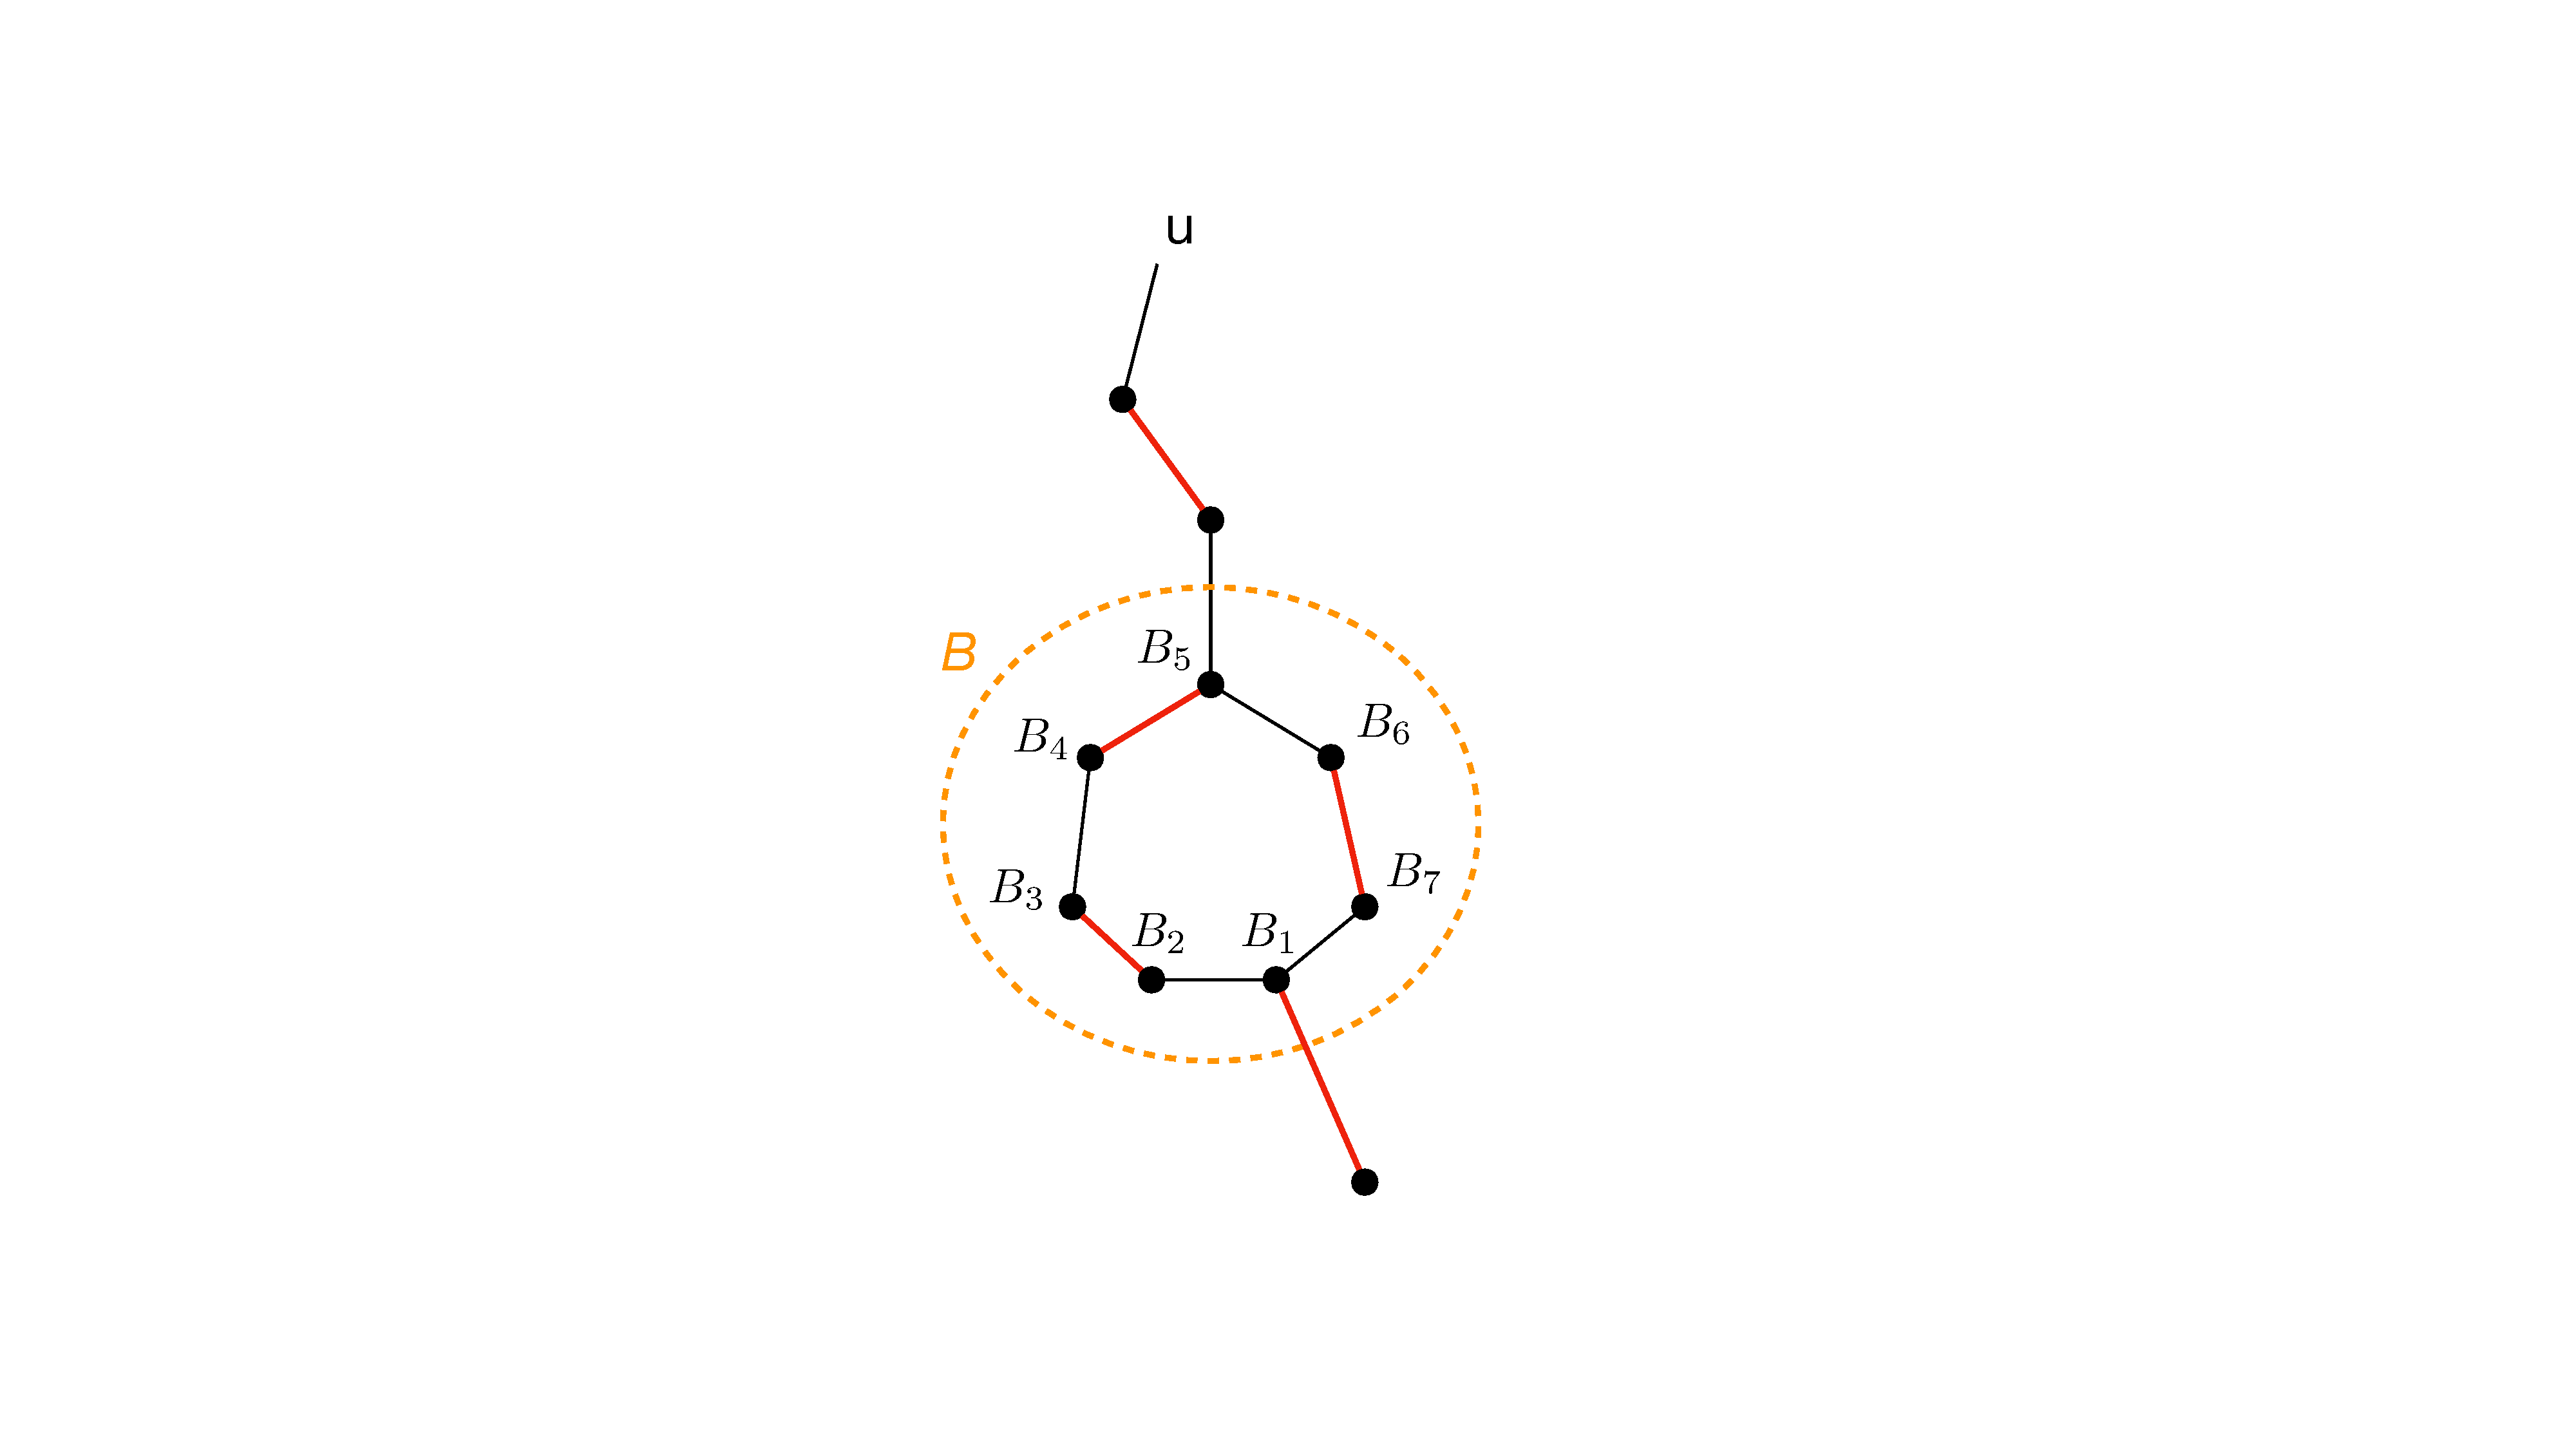
\includegraphics[width=5cm]{fig/lecture_matching_dissolve}
		\caption{In this example, after dissolving blossom $B$ which is drawn as the orange cycle, we keep $B_1, B_2, B_3, B_4, B_5$ in the tree $T_u$, and remove $B_6, B_7$ from $T_u$. Since $B_6, B_7$ are no longer in any search trees rooted at free vertices, we would remove their in/out labels.}
		\label{fig:dissolve}
	\end{figure}
	 
	\item \textbf{New tight edges.} Some new tight edges show up. We argue that any new tight edge must connect two out-blossoms in the contracted graph $\mathcal{G}$, or extend some search trees from an out-blossom to an unlabeled vertex, because in-vertices are only raising the vertex labels. Here are three possibilities which are similar to the unit-weight setting.
	
	\begin{itemize}
		\item If a new tight edge connects to some unlabeled blossoms, then extend the search tree via alternating path as much as possible, and label all the blossoms according to their distance parities.
		\item If a new tight edge $e$ connects two out-blossoms from two different search trees, then we can find a new augmenting path. 
		\item If these two out-blossoms $B_1, B_2$ come from the same search tree, then the unique path between $B_1, B_2$ in the search tree together with $e$ form an odd cycle of alternating path, which creates a new blossom; in this case, we contract this new blossom and add it to $\Omega$.
	\end{itemize}
	\item \textbf{Augmentation.} After a sequence of blossom dissolution and new tight edges, there will be a new augmentation at some point. This happens only when we find a tight edge connecting two different search trees $T_1, T_2$. In this case, let us unlabel all vertices contracted in $T_1, T_2$, and flip the corresponding augmenting path.
\end{itemize}

To find the proper value of $\Delta$ such that one of the above events occur, we can set $\Delta$ to be the minimum among the following terms:
$$\min_{s\notin V(M)}\{y(t)\}$$ $$\frac{1}{2}\cdot\min_{B\in\Omega, \text{in blossom}}\{z(B)\}$$
$$\frac{1}{2}\cdot\min_{s, t\text{ are out and in different trees}, (s, t)\text{ is not tight}}\{\wts(s, t) - y(s) - y(t)\}$$
$$\min_{s\text{ is out}, t\text{ is unlabeled}}\{\wts(s, t) - y(s) - y(t)\}$$
The whole algorithm is summarized \Cref{blossom}.

\begin{algorithm}[H]
	\caption{maximum weight matching in graph $G = (V, E, \wts)$}\label{blossom}
	initialize $M\leftarrow\emptyset, y(*)\leftarrow W, z(*)\leftarrow 0, \Omega\leftarrow \emptyset$\;
	\While{$\min_{u\notin V}\{y(u)\} > 0$}{
		\Repeat{
			set $\Delta$ to be the minimum among the four terms we discussed\;
			$y(v)\leftarrow y(v) - \Delta$ for all out-vertices, and $y(v)\leftarrow y(v) + \Delta$ for all in-vertices\;
			$z(B)\leftarrow z(B) + 2\Delta$ for all maximal out-blossoms, and $z(B)\leftarrow z(B) - 2\Delta$ for all maximal in-blossoms\;
			\If{free vertices have zero vertex labels}{
				\textbf{break}\;
			}\ElseIf{some in-blossoms $B$ has zero dual}{
				dissolve $B$ and add sub-blossoms to the search tree\;
			}\Else{
				\tcc{new tight edges appear}
				extend search trees, or find augmentations, or contract out-blossoms\;
			}
		}
		\If{there exists an augmentation}{
			suppose this is due to a new tight edge connecting search trees $T_1, T_2$, then unlabel all blossoms in $T_1, T_2$, and flip the alternating path\;
		}
	}
	\Return $M$\;
\end{algorithm}

\begin{lemma}
	Between every two consecutive matching augmentation, there are at most $O(n)$ events of blossom dissolution and new tight edges.
\end{lemma}
\begin{proof}
	In general, since there are at most $n$ in-blossoms, and blossom dissolution only destroys in-blossoms, so there can be at most $n$ such events; actually, in our algorithm described above, we never create in-blossoms, so there is none of them.
	
	When new tight edges emerge, either we extend a search tree by two more vertices, or contract an out-blossom. Such events could also happen at most $n$ times. This concludes the proof.
\end{proof}

\begin{corollary}
	The total runtime of the algorithm is $O(mn^2)$.
\end{corollary}
\begin{proof}
	Between any two consecutive matching augmentations, there are $O(n)$ events of new tight edges or blossom dissolution. As each event takes $O(m)$ time by scanning all edges, the total time becomes $O(mn^2)$.
\end{proof}

\begin{lemma}
	When the algorithm terminates, it returns a maximum weight matching.
\end{lemma}
\begin{proof}
	Let $M^\star$ be an arbitrary matching. Then, by dual feasibility and that all free vertices have zero duals, we have:
	$$\begin{aligned}
		\wts(M^\star) = &\sum_{(u, v)\in M^\star} \wts(u, v)\\
		&\leq \sum_{(u, v)\in M^\star} yz(u, v)\\
		&\leq \sum_{u\in V(M^\star)}y(u) + \sum_{B\subseteq V, |B|\geq 3 \text{ is odd}}z(B)\cdot \frac{|B|-1}{2}\\
		&\leq \sum_{u\in V}y(u) + \sum_{B\subseteq V, |B|\geq 3 \text{ is odd}}z(B)\cdot \frac{|B|-1}{2}\\
		&= \sum_{u\in V(M)}y(u) + \sum_{B\subseteq V, |B|\geq 3 \text{ is odd}}z(B)\cdot \frac{|B|-1}{2} = \wts(M)
	\end{aligned}$$
	The last equality uses the fact that there are $\frac{|B|-1}{2}$ matched edges in every blossoms $B\in \Omega$. This immediately concludes the proof.
\end{proof}

\begin{remark}
	It is possible to compress every $O(n)$ iterations into a single iteration in $O(m + n\log n)$, like what we did for bipartite graphs. This improvement is rather involved and is detailed in \cite{gabow2018data}.
\end{remark}